\documentclass{udthesis}

\usepackage{minted}
\usepackage{amsmath}
\usepackage[makeroom]{cancel}
\usepackage[english]{babel}
%\usepackage{float}
%\usepackage[hidelinks]{hyperref}
\usepackage{graphicx}
\usepackage{bookmark}
\usepackage{float}

\makeatletter
\providecommand{\toclevel@prefacesection}{0}
\makeatother
\usepackage{silence}
\WarningFilter{caption}{Unknown document class}
\usepackage[style=default,labelfont=bf,format=hang,belowskip=12pt]{caption}
\usepackage[usenames,dvipsnames]{xcolor}
\usepackage{tcolorbox}
\usepackage{tabularx}
\usepackage{array}
\usepackage{colortbl}
\tcbuselibrary{skins}
\usepackage{chngcntr}
\counterwithout{footnote}{chapter}

\pdfoptionpdfminorversion=7

\definecolor{myblue}{RGB}{72,107,123}
\definecolor{myblue2}{RGB}{184,206,216}
\definecolor{darkgreen}{RGB}{0,151,33}

\newcolumntype{Y}{>{\centering\arraybackslash}X}
\tcbset{borderline={0.5mm}{0.0mm}{myblue},sharp corners,width=1.0\textwidth,enhanced,boxrule=0.5pt,fonttitle=\normalsize,
colback=gray!01!white,colframe=myblue,colbacktitle=myblue2,
coltitle=black,center title,shrink tight}

\newcommand{\unt}[2]{\mbox{#1\,#2}}
\renewcommand\theFancyVerbLine{\normalsize\arabic{FancyVerbLine}}

\apptocmd{\sloppy}{\hbadness 10000\relax}{}{}

\usepackage{draftwatermark}
\SetWatermarkFontSize{24.88pt}
\SetWatermarkScale{8}
\SetWatermarkLightness{0.96}

\begin{document}
    %FIXME: add Acknowledgment.
    \title[A Packetized Display Protocol Architecture for Infrared Scene Projection Systems]{A Packetized Display Protocol Architecture for Infrared Scene Projection Systems}
    \author{Aaron Myles Landwehr}
    \type{dissertation}
    \degree{Doctor of Philosophy}
    \majorfieldtrue\majorfield{Electrical \& Computer Engineering}
    \degreedate{Fall 2020}
    \keywords{MWIR, IR Scene Projection, Infrared LED, Superlattice LED, Optimization, High-speed Systems, Framerate, Frame rate, Display Protocols}
    \subject{Doctor of Philosophy in Electrical and Computer Engineering}

    \maketitlepage

    \begin{approvalpage}
    \chair{Jamie D. Phillips, Ph.D.}{Chair of the Department of Electrical and Computer Engineering}
    \dean{Levi T. Thompson, Ph.D.}{Dean of the College of Engineering}
    \provost{Louis F. Rossi, Ph.D.}{Vice Provost for Graduate and Professional Education and \newline Dean of the  Graduate College\par}
    \end{approvalpage}

    \begin{signedpage} % Up to 4 signatures
        \profmember{Fouad E. Kiamilev, Ph.D.}
        \member{Chase J. Cotton, Ph.D.}
        \member{Xiaoming Li, Ph.D.}
        \member{St\'ephane Zuckerman, Ph.D.}
    \end{signedpage}

    \begin{front} % Starts front material (Roman style page numbers)
        %FIXME: Ack and Disclaimer
        \prefacesection{Acknowledgments}
            I would like to thank my committee for agreeing to be on my committee. I would also like to thank my colleagues who helped with the endeavor of realizing PDP on actual hardware: Andrea, Chris, Daniel, and Tyler. I would also like to thank the rest of my colleagues past and current who helped in any way with PDP through their actions: Alex, Alexis, Andrew, Ben, Casey, Garret, Hamzah, Jaclyn, Jake, Jeff, Johnny, Jon, Josh, Kassem, Katie, Matt, Matt2, Mateo, Michelle, Miguel, Mike, Peyman, Rebekah, Rodney, Spencer, Tianne, Zack.

I would also like to thank my friends who supported me over the years: Angela, Diego, Laura, Jose. I would also like to thank my family who supported me over the years: Joshua and my mom.

Finally, I would like to thank these animals: Aurora, Chowder, Europa, Hal, Hazel, Kiddles, Kosmo, Mewist, Molly, Muffin, Pumpkin, Snickers, Tachi, and these unnamed animals: Birds, Fish, Furbies, Kittens, Mama Cat, Puppies, Random Animals, Tamagotchis.

            The work discussed within this dissertation was partially funded by (a) Air Force STTR Program AF18A-T017 `Next Generation Infrared Scene Projectors for Testing MWIR Systems' (Contract FA8650-19-C-1948), and (b) the Test Resource Management Center (TRMC) Test and Evaluation/Science \& Technology (T\&E/S\&T) Program through the US Army Program Executive Office for Simulation, Training, and Instrumentation (PEO STRI) under Contract No. W900KK-13-C-0049. I thank ONSemiconductor for fabricating silicon arrays, Firefly Photonics and the University of Iowa for fabricating Infrared LED arrays, and Teledyne Scientific for hybridizing Silicon and LED arrays. Their fabrication effort enabled us to build and test the projector system(s) described in this dissertation.
        %\tablespagefalse
        \maketocloflot
        \prefacesectiontoc{Abstract}
            Current fixed frame-rate display technology, such as, DVI, HDMI, and DisplayPort is commonly utilized for high-speed IR display systems. This technology, designed for relatively low-speed operation, incorporates a number of design decisions that limit the ability for it to meet the increasing requirements of larger resolutions and faster framerates needed within IR display systems. Firstly, it requires custom designed synchronization solutions and hardware when utilized within environments where multiple components need to be synchronized. This is because it is not designed to handle system level synchronization. Secondly, the fixed frame rate nature of the technology imposes a static requirement on frame rate across all displayed frames. This unnecessarily increases bandwidth demands by requiring the same amount of data be sent for all frames regardless of what data changes. As a result, maximum frame rate unnecessarily becomes a function of limited hardware bandwidth and image resolution.

This dissertation introduces a generalizable, dynamic, and scalable packetized display protocol (PDP) architecture. It incorporates dynamic frame rates, and high-speed capabilities to bridge the performance gaps within existing display solutions for current IR display systems. This PDP architecture eschews with many assumptions found in traditional display protocol technology. In doing so, it provides scalability, reduces bandwidth requirements, increases performance, eases synchronization burden, as well as, provides a desirable set of features for current and future IRLED Scene Projection systems. These features include dynamic sub-window (intra-frame) refresh rates, dynamic bandwidth utilization, and dynamic inter-frame refresh rates. Furthermore, this dissertation contributes a protocol specification and implementation on real hardware, coupled with, a demonstration of the benefits of this type of technology for use within high-speed IR display systems.

    \end{front}

    \pagenumbering{arabic}

    \chapter{Introduction}
        \label{chap:introduction}

Infrared Scene Projection Systems (IRSPs) are emerging as a novel technology for the testing and development of Infrared (IR) based sensor technology and real-time IR simulations. They provide a compelling alternative to the older entrenched technology of resistor-array based IR scene projector systems~\cite{PritchardEtAl1998,WilliamsEtAl2005} due to various improvements over the competing technology. These improvements include but are not limited to better maximum apparent temperature\footnote{The temperature a black body giving the same radiance would be.} (above 1400 Kelvin), better dynamic range, higher pixel density (24 micrometers and lower), substantially faster emission in the target spectrums with optical rise-times in the nanoseconds. Additionally, they are relatively difficult to damage thermally and have the potential to provide emission in multiple spectrums with \emph{multi-color pixel} designs.

Current fixed frame rate display technology, such as, DVI~\cite{DDWG1999}, HDMI~\cite{HDMIForum2018}, and DisplayPort~\cite{BhowmikEtAl2012} is commonly utilized for high-speed IRSPs. It provides a standardized method to transmit digital scene data which is then translated into analog signaling for display on IR arrays. However, within IRLED IRSP systems which are inherently fast and primarily limited by the driving electronics, it has become limiting for high-speed display~\cite{LaVeignePrewarski2013}. This technology, designed for relatively low-speed operation, incorporates a number of design decisions that limit the ability for it to meet the increasing requirements of larger resolutions and faster frame rates needed within IR display systems. Firstly, it requires custom designed synchronization solutions and hardware when utilized within environments where multiple components need to be synchronized. This is because it is not designed to handle system level synchronization. For example, a display wall may utilize Quadro Sync Cards~\cite{NVIDIA2020_2} to provide synchronization across multiple monitors; however, this only guarantees a coarse-grain synchronization between displays. Secondly, the fixed frame rate nature of the technology imposes a static requirement on frame rate across all displayed frames. This unnecessarily increases bandwidth demands by requiring the same amount of data be sent for all frames regardless of what data changes. As a result, maximum frame rate unnecessarily becomes a function of limited hardware bandwidth and image resolution. This relationship between frame size and bandwidth is discussed in more detail in Chapter~\ref{chap:problem_formulation}.

This dissertation proposes an alternative to traditional display technology, a packetized display protocol (PDP) architecture capable of providing a synergy with IRSP technology to bridge the performance gaps within existing display solutions for current IR display systems. Sensor technology can operate in ranges of above one kilohertz which represents an order of magnitude difference to the current target speeds of fixed-rate display technology. This PDP architecture eschews with many assumptions found in traditional display protocol technology. In doing so, it provides scalability, reduces bandwidth requirements, increases performance, eases synchronization burden as well as provides a desirable set of features for current and future IRLED Scene Projection systems. These features include dynamic sub-window (intra-frame) refresh rates, dynamic bandwidth utilization, and dynamic inter-frame refresh rates. Furthermore, this dissertation contributes a protocol specification and implementation on real hardware, coupled with a demonstration of this type of technology within real IRSP systems which shows that with the proper set of control and features, high-speed operation can be achieved even with limited physical bandwidth.

The protocol architecture draws inspiration from the video processing field, where encoding schemes for video streaming represent a body of research that attempts to tackle a similar but more limited challenge~\cite{BakarEtAl2017}. Some of these encoding schemes attempt to provide a variable frame rate for segments of the incoming stream through differencing algorithms, but also rely on compression~\cite{CastilloEtAl2012} which reduces quality and introduces artifacts. In contrast, the case of IRSPs requires lossless quality; and thus, lossy protocols cannot be utilized for this purpose. Instead, the proposed protocol architecture seeks to craft a lossless solution for the IRLED projector field that incorporates similar variable frame rate features to reduce bandwidth consumption as well as allow bandwidth to be used more intelligently. More specifically, it is envisioned that available bandwidth will be apportioned to regions of a scene that necessarily need to be updated frequently. In IR scenes, this generally includes regions that transition from dark to light or light to dark quickly, as well as higher temperature regions. Regions which do not change temperature quickly, generally do not need to be updated as often due to the LED driving circuits holding capacitance for milliseconds at a time\footnote{The general time of discharge depends on the design of the LEDs and amount of charge currently held within. However, test setups have measured \textgreater1 millisecond.}.

The contributions of this dissertation are as follows: firstly, it provides the architecture of a physical layer agnostic packetized display protocol with the following features: (1) intelligent dynamic per-frame bandwidth utilization, (2) fine-grained control over frame transmission and synchronization, (3) dynamically changing intra-frame rates, and (4) a realized implementation of the protocol for use on array emitter technology. Within it discusses relevant details of the initial design, methodology, and implementation of the said protocol. Secondly, it provides a sufficiently abstract machine model to indicate a path to utilize the protocol within current and future systems. Thirdly, it demonstrates the use of the protocol within real IRSP systems as well as provides the current results and a comparison with fixed-rate technology. Fourthly, it discusses various use cases for the technology to provide the reader with a more complete understanding of where this technology could be utilized in future systems.

The rest of this dissertation is divided into the following sections: (1) background; which discusses the various aspects of current IRSP systems that are relevant to understanding the IRLED scene projector history and projection process, (2) problem formulation; which examines the problem of high-speed projection in detail, (3) system overview; which discusses the supporting electronics and communication flow within IRLED projector systems, (4) array write process; which discusses how IR arrays and the associated data ordering, (5) display protocols; which discusses conventional display protocols and their use within IRSP technology, (6) packetized display protocol; which discusses the design methodology for the PDP, packet details, overhead, and performance, as well as provides a comparison to conventional display protocols; (7) machine model; which discusses the use of the PDP in general systems; (8) implementation; which discusses an implementation of the PDP on an FPGA system, (9) experimental results; which provides details on the implementation and testing process as well as a discussion on performance; and (10) conclusion; which discusses the future of PDP and potential avenues of further research.

    \chapter{Background}
        \label{chap:background}

    This chapter discusses relevant background information toward the goal of implementing a packetized display protocol (PDP) architecture for Infrared Scene Projector systems (IRSPs). First, it gives an overview of what constitutes an IRSP system. Following this, it provides a general discussion of how common display protocols work to send pixel data to a display system (e.g. a television). Finally, it discusses how these protocols are utilized within an IRLED project system including discussion of example scenarios.

\section{IRLED Projector Systems}

    \begin{figure}
        \centering
        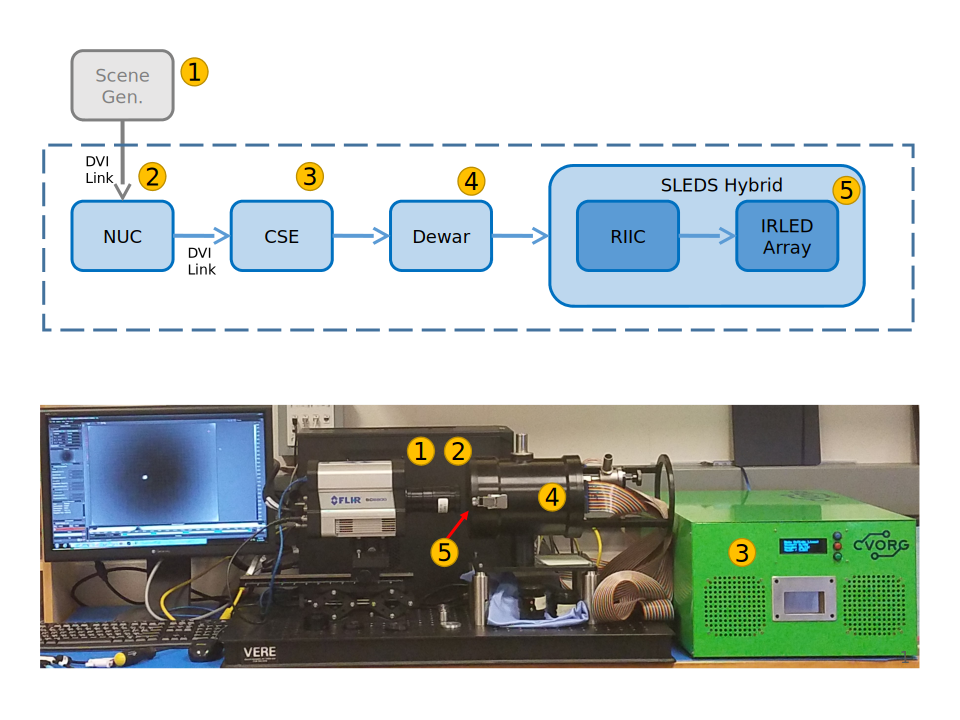
\includegraphics[width=1.0\textwidth]{fig/sleds_system.pdf}
        \caption{IRLED Scene Projector System}
        \label{fig:sleds_system}
    \end{figure}

    IRLED based IRSPs are made up light emitting diodes (LEDs) that emit light in the IR spectrum\cite{biard1966semiconductor}. Since their inception they have been utilized in various fields such as medical\cite{MonteiroEtAl2011,MEEKS1998433,Sadick2009,takhtfooladi2015effects,yamanishi1995respiration} sensing; tracking; and localization\cite{PlotogVladescu2015,Kimon2001,SCHOLZ20151233,WalshDaemsSteckel2015,zeylikovich2003mid}, and communication\cite{CossuEtAl2014,escobosa2004ir,GeorgopoulosKormakopoulos1986,sohn2007localization,JangEtAl2012}. Modern IRLED projectors are an emerging technology with various applications within the IR sensor testing community. A complete IRLED based IRSP system consist of various technologies and processes as shown in Figure~\ref{fig:sleds_system}. One denotes the scene generation and non-uniformity correction (NUC) process. This is where pixel data representing IR scenes is fed to a system for display. The NUC process is for correcting for physical and thermal non-uniformity\cite{BarakhshanEtAl2017} in an IRLED array\cite{BarakhshanEtAl2018}. Two denotes the close support electronics\cite{ejzak4} which are responsible for converting a digital representation of a scene into analog signaling that goes directly to an array. Three indicates the dewar\cite{lang1, MarksEtAl2017} or vaccum chamber which houses an IRLED array and is utilized to keep it below ambient temperatures or at cryogenic temperature ranges. Four indicates an IRLED hybrid which consist of a Read-in Integrated Circuit (RIIC)\cite{HernandezEtAl2017} used to address an IRLED array and the array itself. Analog signals coming from the CSE go into the dewar, and then are mapped using the RIIC, which results in specific IRLEDs within an array being driven. Five indicates an IR recording apparatus of some sort utilized to record IR data from an array. Synchronization between source generation, display, and recording is maintained via synchronization signaling. Often Camera Link serial communication\cite{CameraLink2000, zhu2008design} is used.


    Figure~\ref{fig:sleds_timeline} shows the development timeline for IRLED Projector technology. In 2008, the world's first IRLED array called the Superlattice Light Emitting Diodes (SLEDs) array was completed in 2008\cite{ahmed1}. This device was a hybridized combination of an 68 by 68 IRLED wafer bonded to a RIIC wafer\cite{das2} providing the electronics to drive the array. Initial testing was done by hand prior the design and implementation of the overall drive system was completed in 2011. Following this, an increased IRLED wafer of 512x512 size was fabricated in 2014\cite{norton1}. These efforts culminated in the first two IRLED projector systems in 2016. The first, TCSA (Two Color SLEDS Array), a 512 by 512 sized array\cite{McGeeEtAl2015, ejzak1, ejzak2, EjzakEtAl2016, RickerEtAl2017} included support for driving the LEDs at two separate wavelength bands (denoted as 2-colors in Figure~\ref{fig:sleds_timeline}. The second, NSLEDS (N Superlattice Infrared Light Emitting Diode System), a 1024 by 1024 sized array\cite{benedict1} doubled the total number of pixels supported. Additionally, these systems demonstrated the beginnings of a modular IR Scene Projection (IRSP) platform\cite{BrowningEtAl2019}. A further increase in size and efficiency occurred in 2018 with the world's first 2048 by 2048 pixel array, HDILED (High Definition Infrared LED). A visual representation of the pixel ratios is shown in Figure~\ref{fig:tcsa_nsleds_hdiled_array_ratio}

    \begin{figure}
        \centering
        \includegraphics[trim=0.5in 0.5in 0.5in 1.5in,width=1.0\textwidth]{fig/sleds_timeline.pdf}
        \caption{IRLED Projector Technology Development Timeline Overview}
        \label{fig:sleds_timeline}
    \end{figure}

    \begin{figure}
        \centering
        \includegraphics[trim=0.5in 0.5in 0.5in 1.5in,width=1.0\textwidth]{fig/tcsa_nsleds_hdiled_array_ratio.pdf}
        \caption{SLEDs Array Pixel Ratios}
        \label{fig:tcsa_nsleds_hdiled_array_ratio}
    \end{figure}

    TCSA represented a novel step forward in terms of IRLED array technology. It incorporated a multiple color pixel design to enable emission in multiple wave-length spectrums, as well as, an increase in the number of analog channels from 4 to 16 to allow for more pixels to be driven at a time. NSLEDS used the same size wafer as a TCSA, but incorporated only a single-color pixel design instead of the multiple color design of the original, which allowed for the pixel resolution to be doubled paving the way toward larger format SLED IRSPs. HDILED combines. The interleaved write process of each array will be discussed in detail in Section~\ref{sec:array_Interleaved_write_process}.

    Figure~\ref{fig:typical_projection} shows a typical projection process utilized within an IRLED system. A scene projector will perform scene generation utilizing a GPU typically. Following this, imagery will be undergo non-uniformity correction by utilizing a NUC table created by analyzing the non-uniformity on a given array. This process compensates for any physical defects that may cause non-linear variation in light emission from different diodes on a given array, thus, allowing for uniform emission across a given spectrum. There are number of different ways this linearization may be performed\cite{BrowningEtAl2016, LandwehrEtAl2017, BarakhshanEtAl2019}, but that is beyond the scope of this work.

    \begin{figure}
        \centering
        \includegraphics[trim=0.5in 0.5in 0.5in 1.5in,width=1.0\textwidth]{fig/typical_projection_system.pdf}
        \caption{Typical IRLED Projection Process}
        \label{fig:typical_projection}
    \end{figure}


    %FIXME: add discussion about the speeds

    %FIXME: add discussion about uses

    %FIXME: add discussion about system layout

\section{Classical Display Protocols}
    \label{sec:classical_display_protocols}

    Classical display protocols such as (DVI\cite{DDWG1999}, HDMI\cite{HDMIForum2018}, and DisplayPort\cite{VESA2016} are commonly used for driving consumer electronic devices. These generally provide a standardized feature-set that is rooted in classical analog video specifications (e.g. VGA, Composite)\cite{NIAnalog} that utilize scan lines\cite{Neal1998}. Scan lines are used to provide video timing information in order to synchronize a display to a given refresh-rate. Each scan line consist of an active video region followed by a horizontal blanking period. After all active video scan lines are displayed, a vertical synchronization region is used to indicate the end of a frame.

    \begin{figure}
        \centering
        \includegraphics[width=0.9\textwidth]{fig/display_timing_overview.pdf}
        \caption{Display Protocol Timing Overview}
        \label{fig:display_protocol_timing_overview}
    \end{figure}

    \begin{figure}
        \centering
        \includegraphics[width=0.7\textwidth]{fig/display_timing_line_cross.pdf}
        \caption{Display Protocol Horizontal Signal Cross Section Timing}
        \label{fig:display_protocol_line_cross}
    \end{figure}

    %FIXME add crosssectional blowout chart

    An overview of this is shown in Figure~\ref{fig:display_protocol_timing_overview}. The region shown in green is the pixel data for the active video region of the display. It is of size $H_a\times V_a$ which represents the number of pixels to display, for example, 1920 by 1080 for a HDTV high-definition video mode\cite{MythTVWebsite}. The blanking time regions denote pixel data that is sent but not displayed\footnote{Typically data lines are held low during this period, but somtimes it is used for out-of-band communication to send other information such as audio encoding.}. A scan line consist of pixels made up of $h_a$, the horizontal active size; $h_{fp}$, the horizontal front porch before the pulse signal; $h_{sp}$, the horizontal sync pulse; and $h_{bp}$, the horizontal back porch after the sync pulse. The vertical blanking period makes up multiple scanlines and consist of $v_{fp}$, the vertical front porch before the vsync pulse; $v_{sp}$, the vertical sync pulse; $v_{bp}$, the vertical back porch after the vertical sync pulse. Sync pulses are generally active low, meaning that during active display a sync signal is high as shown in the diagram.

    Figure~\ref{fig:display_protocol_line_cross} shows a closeup view of signal lines during the active region of display for two scan lines. A data enable signal denoted by $enable$ is high during the active region shown in green. Following this, it goes low for a period of time denoted by $h_{fp}+h_{sp}+h_{bp}$. The horizontal sync signal goes low only in the region shown in yellow between the front porch and back porches. This process repeats for all scan lines. Once the last active region pixel is drawn, the enable signal will stop going high during the vertical synchronization period.

    %FIXME: Fix discussion of DP not using fucking backwards compatibility shitty hdmi fucking mode
    %FIXME: Talk about CC in the vertical blanking

    \begin{figure}
        \centering
        \includegraphics[width=0.9\textwidth]{fig/display_timing_full_cross.pdf}
        \caption{Display Protocol Full Signal Cross Section Timing}
        \label{fig:display_protocol_full_cross}
    \end{figure}

    Figure~\ref{fig:display_protocol_full_cross} shows a closeup view of signal lines during the transition into the vertical synchronization period. The region donated by $V_a$ indicates the end of the video active region of the display which occurs toward the end of a frame. After the active video region, all data has been drawn to a display. The region denoted by $v_{fp}+v_{sp}+v_{bp}$ is the vertical blanking or vsync period during which no active video data is sent; therefore, data enable denoted by $enable$ is always low during this period. Before the vertical sync pulse period denoted by $v_{sp}$ occurs, a vertical front porch period denoted by $v_{fp}$ occurs. After the vertical sync pulse, a vertical back porch region $v_{bp}$ occurs. Following this the beginning of the next frame occurs as denoted by $v_{a+1}$.
    \begin{figure}
        \centering
        { \Large
            $l_h=h_a+h_{fp}+h_{sp}+h_{bp}$ \vspace{8px} \\
            $l_v=v_a+v_{fp}+v_{sp}+v_{bp}$ \vspace{8px} \\
            $f_f={f_p \over {l_h \cdot l_v}}$ \\
            $p_t={1 \over f_p}$ \vspace{8px} \\
            $f_t={1 \over f_f}$ \vspace{8px}
        }
        \caption{Total Refresh Rate}
        \label{fig:modeline_refresh_rate}
    \end{figure}

    Figure~\ref{fig:modeline_refresh_rate} shows the relationship between between the different regions of a display and the frequency or refresh rate. $l_h$ denotes the scan line size of a display, or total horizontal width, which is made up of the horizontal active and horizontal porch region pixels of a display. $l_v$ denotes the total vertical width of a display, which is made up the vertical active and vertical porch region pixels of a display. Each pixel is sent at a rate denoted by $f_p$, the pixel frequency (also called the pixel clock). $f_f$ denotes the frame frequency or framerate of a display. This is simply the pixel frequency over the total number of pixels (video active and porches) of a display. $p_t$ denotes the time period a single pixel takes to send. $f_t$ denotes the time period for an entire frame.

    %FIXME: example modeline
    To illustrate, let us look at the display modeline generated using the VESA Coordinated Video Timing (CVT) standard shown in Figure~\ref{fig:modeline_example}. This modeline operates a total frame frequency of approximately \mbox{30 Hz}. The pixel clock 79.75, denoted in red, is specified in megahertz. The horizontal pixels, denoted in blue; are the end of horizontal active, the end of horizontal front porch, the end of horizontal sync pulse, and the end of horizontal back porch respectively. The vertical pixels (measured in lines), denoted in green; are the end of vertical active, the end of vertical front porch, the end of vertical sync pulse, and the end of horizontal back porch respectively. The sync pulse polarities, denoted in yellow; indicate whether a given sync pulse is active low or active high. A minus symbol indicates active low and a plus symbol indicates active high. If these numbers are placed into into the formulas shown in Figure~\ref{fig:modeline_refresh_rate} the results shown in Figure~\ref{fig:modeline_refresh_rate_plug} are yielded. The astute reader will note that $l_h$ and $l_v$ are the same as the total pixel size for the given modeline. The pixel period is $\sim12.53 ns$, meaning that each pixel is drawn for the given amount of time. The frame period is $\sim33.33 ms$, meaning that each frame is drawn for that given amount of time.

    \begin{figure}
        \centering
        { \normalsize
        \textbf{``1920x1080\_30.00"} {\color{red}79.75}  {\color{blue} 1920 1976 2168 2416}  {\color{darkgreen}1080 1083 1088 1102} {\color{olive}-hsync +vsync}
        %\vspace{-8px}
        }
        \caption{VESA CVT Generated Modeline}
        \label{fig:modeline_example}
    \end{figure}

    %FIXME: finish this chart
    \begin{figure}
        \centering
        { \Large
            $h_a=1920; h_{fp}=1976-h_a; h_{sp}=2168-h_{fp}; h_{bp}=2416-h_{sp};$ \\
            $v_a=1080; v_{fp}=1083-v_a; v_{sp}=1088-v_{fp}; v_{bp}=1102-v_{sp};$ \\
            $l_h=2416=1920+56+192+248$ \vspace{8px} \\
            $l_v=1102=1080+3+5+14$ \vspace{8px} \\
            $f_p=79.75e6$ \vspace{8px} \\
            $f_f=30.0={f_p \over {l_s \cdot l_c}}$ \\
            $p_t=12.53ns={1 \over f_p}$ \vspace{8px} \\
            $f_t=33.33ms={1 \over f_f}$ \vspace{8px}
        }
        \caption{Computed Refresh Rate for a 30hz CVT Modeline}
        \label{fig:modeline_refresh_rate_plug}
    \end{figure}

    Section~\ref{sec:displays_within_proj_system}, discusses how these protocols are utilized within an IRLED projector system, briefly highlight the limitations, and . %FIXME: finish this paragraph

\section{Display Protocols within an IRLED Project System}
    \label{sec:displays_within_proj_system}
    Projector systems utilize

\section{Array Interleaved Write Process}
    \label{sec:array_Interleaved_write_process}
    As discussed in Section~\ref{sec:classical_display_protocols}, while all current IRSP arrays utilize some display protocol technology that is decoded in order to drive an array's pixels, they may utilize different internal drawing mechanisms for driving the pixels. This section discusses the details of those mechanisms within the NSLEDs and HDILED arrays for conceptual purposes, and while the details may differ for other arrays, the raster write process will be similar.

    The NSLEDs and HDILED arrays are organized into four quadrants as shown in Figure~\ref{fig:tcsa_nsleds_hdiled_quads}. Internally each quadrant has separate internal signaling.

    \begin{figure}
        \centering
        \includegraphics[trim=0in 0.35in 0in 1.5in,width=1.0\textwidth]{fig/tcsa_nsleds_hdiled_quads.pdf}
        \caption[TCSA, NSLEDs, and HIDLED Array Quadrant Layouts]{TCSA, NSLEDs, and HIDLED Array Quadrant Layouts\textsuperscript{a}}
        \vspace{-8px}
        \footnotesize\textsuperscript{a} Not drawn to scale
        \label{fig:tcsa_nsleds_hdiled_quads}
    \end{figure}

    \chapter{Problem Formulation}
        \label{chap:problem_formulation}

This chapter discusses in detail the limitations with current display protocol technology that were alluded to in Chapter~\ref{chap:introduction}. From there, it focuses on how these limitations affect adversely IRLED projector technology. Finally, it provides a problem solution.

\section{Display Protocol Limitations}

    % FIXME: Reference display protocol background section here

    Current display technologies, such as HDMI, assume a fixed frame rate display which places a hard limit on frame timing and synchronization.

    % Limitations:
    % Synchronization:
    %   -Implementation and integration-costs $
    %   -System-specific solutions $
    %   -Poor upgradeability $
    In detail, display protocols operate in a best-effort fashion where a buffer swap initiated transfer of frame data occurs at a static predetermined interval. If a new frame is unavailable to be transmitted at each interval due to any delay, such as processing delay, the previous frame will be retransmitted. This necessarily makes correct synchronization challenging because modern computation systems do not generally provide real-time guarantees for several reasons, such as, variability in system operation, including frame generation, CPU scheduling, and Input/Output (I/O) delays. Generally, while these challenges can often be addressed to some degree, they require custom hardware solutions on top of existing display protocols because end-to-end system synchronization is out of the scope of typical display standards which are designed to push relatively low frame rates over single hardware links. These solutions also tend to lack abstraction layers which can greatly hinder upgradeability.

    % Limitations:
    % Display Protocols
    %   -Frame rate limits                 -> image size inversely proportional to speed $
    %   -Static Bandwidth Requirements     -> full image transfer $
    %   -Static frame rates                -> 60Hz, 100Hz, etc. $
    %   -Scalability                       -> single scene generator, projector driver $
    %   Diagrams: Bandwidth diagram -- referenced already $
    Moreover, because of the static nature of the transmission interval (e.g. 100Hz), the frame rate cannot be dynamically controlled or changed after initialization. Instead, these protocols have static bandwidth requirements for a given resolution and frame rate of the form found in Table~\ref{tbl:bandwidth}, which shows that image size is inversely proportional to the max speed the display can operate at. Additionally, these protocols only support sending the entire frame at a given interval even if only a small portion of the frame has changed. This is a non-optimal use of bandwidth that does not allow for fine-grained control over the frame rate in cases where a user might wish to dynamically change the frame rate to match the processing rate. In high-speed display scenarios, this inevitably causes dropped frames. This issue is further compounded by the fact that traditional display protocols utilize proprietary drivers and hardware such that frame-drops become effectively silent. Similarly to the synchronization solutions discussed above, this tends to lead to upgradeability issues due to systems being tailored for specific display hardware. This contributes to scalability issues as well since changing the display hardware often requires a complete system redesign.

    % Analog Chain:
    %   -RT settling time limitations: -- not included right now
    % Existing diagrams:
    %   Diagrams: scene generator -> Non-uniformity Correction -> Projector
    %   Diagrams: Modeline Overhead diagram

    \begin{table}
        \centering
        \large
        %\begin{small}
        %$$bandwidth = resolution \times bits \times fps$$
        %$bandwidth$ : \quad bandwidth requirements in bits per second. \\
        %$resolution$ : \quad number of pixels including porches. \\
        %$bits$ : \quad \quad \quad \ \ \ bits per pixel. \\
        %$fps$ : \quad \quad \quad \ \ \ frames per second.
        \begin{tabular}{| r l |}
            \hline
            $bandwidth$ & = resolution $\times$ bits $\times$ fps \\ \hline
            $bandwidth$ & : bandwidth requirements in bits per second. \\
            $resolution$ & : number of pixels including porches. \\
            $bits$ & : bits per pixel. \\
            $fps$ & : frames per second. \\
            \hline
        \end{tabular}
        \caption{Bandwidth requirements of a traditional display protocol}
        \label{tbl:bandwidth}
        %\end{small}
    \end{table}

\section{High-speed IRLED Projector Systems}
% How these limitations affect IRSP
% Bottlenecks:
% Hardware limitations:
%   -Physical interconnect bandwidth and latency -> Concurrency/Parallelization $
%   -FPGA/ASIC/IC clock rates                    -> Concurrency/Parallelization $
%   -Analog chain settling times (DAC)           -> Address only the pixels needed $
% Software limitations:
%   -Computational/algorithmic limitations       -> Concurrency/Parallelization $
%   -Poorly optimized software / drivers         -> Do not use $
%   -Fixed frame display                         -> Dynamic frame rate + frame segmentation $
%   -Non-RT scheduling                           -> Realtime schedule / DMA -- not covered below - do i want to cover this?
%   -Lack of control                             -> Use a communication protocol with dynamic control built-in $
%

%FIXME: stick section BLAH in
    In the field, these conventional display protocols, which are designed for driving relatively low speed consumer electronics as indicated in Chapter~\ref{chap:display_protocols}, are often utilized in High-speed IRLED Projector systems. This results in a combination of unnecessary hardware and software limitations being incorporated into systems. This section will discuss these limitations and the general methodology toward alleviating them. Hardware limitations will be discussed followed by software.

    \subsection{Hardware Limitations}
        There are several hardware limitations including physical bandwidth, latency, IC clock rates, and analog chain settling times. Often the hardware that data is transferred over within these systems has inherent bandwidth and latency limitations that cannot be overcome either due to the nature of physics or simply because faster hardware is not available. One solution toward working around bandwidth issues is to introduce more parallel links into a system. A similar issue arises with respect to the clock rates of components within a system, such as, projector driver firmware, and scene generator. Ideally, these components will operate as fast as possible, but the reality is that the large fan out of I/O signaling needed by arrays can cause critical timing closure issues within FPGA based firmware implementations. Careful routing and planning can help alleviate these issue as well as parallelizing projector drivers such that less signals are driven from a single FPGA component. The speed of the analog chain in these systems is dictated by the digital to analog converter (DAC) and amplifier settling times which can be alleviated by increasing the number of converters utilized within a system if supported by an array. This could increase write speeds by allowing more DACs and amplifiers to drive smaller portions of an array in parallel. All the solutions discussed in this section involve increasing the amount of parallelized components operating within a system in order to reduce physical bottlenecks.

    \subsection{Software Limitations}
        In terms of software, computational and algorithm limitations exist in the generation of scenery for display, and in correcting for pixel and array imperfections as well as in putting data in the correct format to be understood by a projector's driving firmware. Rendering of individual frames of a scene can be particularly computationally expensive. This can be further complicated by poorly optimized software drivers or algorithms. Additionally, in these systems, tight control over timing is important because frame drops are not tolerable. Meaning that fixed rate display technology is a hinderance in terms of user level control. One solution is to utilize technology that allows for dynamic frame rates and frame segmentation, which, requires protocols with dynamic control built in.


\section{Problem Statement}
    IRSP systems need to be capable of operating at high speeds with large resolutions to meet the needs of the sensor testing community. Typically, this can be on the order of 2048 by 2048 pixels with up to 1KHz frame rates with subframe latency. Necessarily, these goals represent a challenging problem to overcome when utilizing typical display technology which is further hindered due to the limitations discussed above. Given these constraints, the question of what is an appropriate solution to address the aforementioned issues arises. The central question we could ask ourselves is, how to architect a generalizable, dynamic, and scalable IRSP system capable of High-performance operation, sub-frame latency, dynamic frame rates, and dynamic bandwidth utilization?

\section{Problem Solution}
    Within the current display protocol technology, any effort to address the aforementioned issues requires system developers to have complete control over an entire end-to-end system for a given solution to operate correctly. This means that in practice customized hardware and software that deviates from the standard display protocols behavior is required. Any solution that lacks these requirements would fail to completely address operational issues with performance.

    In short, to truly address issues within the traditional display protocol would require creating a new system specific protocol tied to specific custom hardware. Additionally, with this type of solution, it is still not possible to achieve true sub-frame latencies due to the nature of display protocols requiring transmission of entire frames of data at a given interval or frame rate. In practice, IR projector systems are typically forced to introduce intermediate buffers within a system in order to ensure correct operation.

    I believe that any effort to address the aforementioned issues and answer our problem statement requires developing an alternative display protocol designed specifically for high-speed low latency frame transmission as well as is hardware agnostic in nature, and utilizable within different types of hardware setups. This would allow for the protocol be retrofitted within existing systems as well as allow for upgradeability, and support for future hardware. In order, to achieve sub-frame latencies, this protocol would need to support transmission of sub-frames of data, i.e. transmission of partial frames. Allowing for partial frame transmission enables a host of other desirable features, such as, the ability to control bandwidth utilization and the ability to incorporate dynamic frame rates. A good method of supporting partial frame transfer is to utilize headered packets of data to provide a context for what the data represents and where to draw said data on a display. This method of transferring display data is called a packetized display protocol (PDP).

    As discussed briefly in the Chapter~\ref{chap:introduction}, this PDP architecture eschews with assumptions found in traditional display technologies to provide a robust feature-set. This section discusses many of the assumptions of traditional display technologies and how the PDP architecture differs to provide the reader with an understanding of the benefits to the proposed alternative technology.

    In contrast to a normal display protocols, the proposed architecture, is designed to utilize a dynamic source driven refresh rate through the coordination of both source (scene generator) and sink (display). In this architecture, frames are segmented into pieces and sent to the display based upon how often these segments need to update. An example of this is shown in Figure~\ref{fig:variable_display} where different regions of the display operate at different frame rates. By utilizing dynamic frame rate control at sub-frame resolutions, substantial bandwidth reductions can occur. This will be discussed in further detail in subsequent chapters.

    \begin{figure}
        \centering
        \includegraphics[width=1.0\textwidth]{fig/variable_display.pdf}
        \caption{Dynamic frame rate display with multiple regions updating at different frame rates}
        \label{fig:variable_display}
    \end{figure}

    %FIXME: what mechanisms to synchronize displays?
    As will be discussed in Chapter~\ref{chap:pdp_protocol}, the underlying PDP itself is designed to allow for fine-grained control over when and what data is transmitted as well as to incorporate mechanisms to synchronize displays. Furthermore, the protocol architecture is abstracted in such a way that the physical interconnect layers are transparent in order to enable it to be capable of operating over a wide-spectrum of hardware as well as to allow the protocol to be extended and used within future hardware. For system upgradeability, this offers a risk reduction because it allows for a simpler migration path as new hardware becomes available. For example, a hardware system implementing this protocol could switch or upgrade physical components and still utilize the same protocol within the software stack given an appropriately compatible physical layer. To further facilitate this, a packetized protocol structure capable of transmitting pixel data in a generalized way has been chosen.

    \chapter{System Overview}
        \label{chap:system_overview}
This chapter provides the reader with an overview of IRLED electronics. Firstly, it discusses the Close Support Electronics (CSE)~\cite{EjzakEtAl2015,HernandezEtAl2019,SinghEtAl2020} hardware used to drive IRSP systems to give the reader an understanding of the internal flow of data from entry into a CSE to output to an external array. Following this, it discusses the communications within a CSE at a block level to provide the reader with an understanding of how communication flow works within a CSE for configuration. Finally, external communication of an overall IRLED system is discussed at a block level to provide the reader with a high-level understanding of the flow of communication from input (scene generation) to output (array) in different system configurations.

\section{Close Support Electronics}
    \label{sec:close_support_electronics}
    As mentioned briefly in Chapter~\ref{chap:background}, a CSE is needed to drive IRLED arrays. Conceptually, A CSE is an interface that converts digital display data to an array specific format in order to produce IR imagery. From there it converts formatted data from the digital domain to analog and amplifies analog signaling to drive an array by charging the internal array cells that make up an array. It further provides power for an array and regulates the current to safeguard arrays from physical damage due to misconfiguration, heating, or hardware faults.

    The TCSA, NSLEDS, and HDILED arrays discussed in Chapter~\ref{chap:background} can all be driven using the same electronics with the only difference in the boards directly attached to the hybrid array. Figure~\ref{fig:sleds_block} shows the internal components of the CSE architecture, called {\it Nessie}, broken out in green. In typical configurations, a display system drives a CSE using dual HDMI inputs to increase the system bandwidth and achieve higher frame rates. Typically, these will each carry half of a frame segmented either vertically or horizontally. Each input decodes the video signals in parallel and then outputs individual pixels that are then routed into the main FPGA board which houses a Xilinx Vertex 6 FPGA~\cite{XILINX2015}. From there, pixels are routed into an internal buffered directly or decoded (in the case of PDP) and then buffered. Other interfaces may be utilized in place of HDMI as will be discussed later in this section.

    \begin{figure}
        \centering
        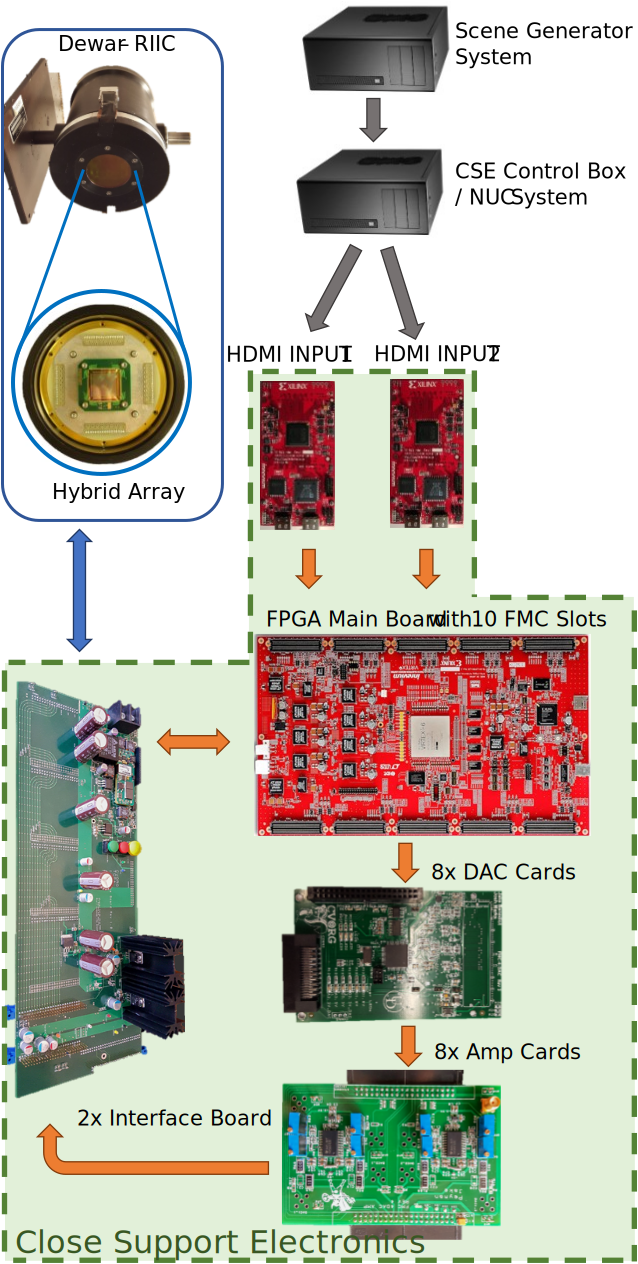
\includegraphics[width=0.67\textwidth]{fig/sleds_block.pdf}
        \caption{SLEDS System Block Diagram}
        \label{fig:sleds_block}
    \end{figure}

    Due to the two input cards, the firmware within the main FPG board is responsible for multiplexing between both inputs to draw data to an array without allowing for the internal firmware buffers to overflow. In practice, current firmware does this by buffering the minimal amount of data needed for a write from both inputs in parallel and context switches between the inputs every other write or every two writes depending on the configuration. As long as the buffers are sized large enough to accommodate for the time needed for the array write process to finish for an individual write, then overflow should not occur. Additional logic is provided to query and detect internal buffer overflows in cases of misconfiguration or signal integrity faults. In practice, if an overflow fault occurs, it is visually obvious in recorded IR data as well.

    Once enough data is buffered for one of the inputs, the firmware will control the write process to drive the 8 DAC cards which each house 2 16-bit DAC integrated circuits per card, with each circuit consisting of 2 channels per DAC. Yielding 32 parallel channels with 512 total signals. Once the DAC process is done, the analog output of the 32 channels is then routed to 8 amplifier card which contain 4 amplifiers each. Following this, the amplified signals are routed through 2 interface boards which contain ribbon cables that attach to an array hybrid. The ribbon cabling carries both the amplified signals as well as other control signals from the firmware that are routed directly from the main FPGA board to one of the interface boards.

    Figure ~\ref{fig:round_board} shows an example of a circuit board which ribbon cables would be attached to via receptacles (not shown). Four ribbon cables can be attached to bring signaling to an array.

    \begin{figure}
        \centering
        %includegraphs[trim=L B R T]
        \includegraphics[width=1.0\textwidth]{fig/round_board.png}
        \caption{Example Hybrid Round Boards}
        \label{fig:round_board}
    \end{figure}

    Figure~\ref{fig:nessie_enclosure_internals} shows the components installed within a CSE chassis. Multicolored ribbon cables are shown in the top right. Mounted to the bottom is the main FPGA board. The two large boards at the top are the 2 interface boards with 8 amplifier cards plugged into them along the bottom. The boards in between the FPGA and amplifier cards are the DAC cards. The power supply is on the left.

    \begin{figure}
        \centering
        \includegraphics[width=1.0\textwidth]{fig/nessie_enclosure_internals.jpg}
        \caption{CSE Internals}
        \label{fig:nessie_enclosure_internals}
    \end{figure}

    The additional control signals provided by the firmware and routed to the RIIC through these cables are discussed in Chapter~\ref{sec:array_Interleaved_write_process}. The specifics of the PDP firmware architectures write process are discussed in Chapter~\ref{chap:implementation}.

    Figure~\ref{fig:nessie_enclosure_externals} provides an external view of a newer CSE chassis that is colored green to follow the {\it Nessie} architecture name as well as a view of the inside of the chassis when the majority of components aren't installed.

    \begin{figure}
        \centering
        \includegraphics[width=1.0\textwidth]{fig/nessie_enclosure_externals.png}
        \caption{CSE Externals and Empty Chassis}
        \label{fig:nessie_enclosure_externals}
    \end{figure}

\section{Communication Flow}
    In this section, a discussion of internal CSE communication will be provided followed by a discussion of external communication within an IRLED projector system as a whole.

    \subsection{Internal CSE Communication}
        Figure~\ref{fig:cse_comm_block} shows the internals of CSE communication. Communication for controlling the behavior of CSE is done through a daisy chained set of UART devices utilizing a reliable blocking two way communication protocol called the CVORG protocol\footnote{Named after my research group at the University of Delaware.}. Without loss of generality, the protocol itself consists of commands to control various aspects of operation, such as, tripping an array, setting voltage limits, and configuring firmware operation. It also allows for information to be retrieved about current system configuration as well as operational errors. The destination of an operation is encoded as part of each command. Thus, commands not meant for a given component are forwarded along the chain. When commands are issued by a system, they are encoded for transport via the CVORG protocol and sent over UART. The system will then wait for an acknowledgment potentially containing payload data. When a command has finished executing within a CSE, it will send the acknowledgment over UART to the command initiator with requested payload data or simply as a receipt indicating that an action has been successfully executed. The underlying implementation details of the CVORG protocol itself are beyond the scope of this work and will not be discussed here.

        Memory mapped I/O between the frontend and backend firmware is controlled by the Microblaze soft processor and used to control the underlying PDP firmware registers as well as program an array using Serial Peripheral Interface (SPI) (Not shown). The details of command operations will be discussed in Chapter~\ref{sec:frontend_arch}. Additionally, SPI communication is also used to send data for LCD readout. Typically, this includes voltage and current information as well as the results of power on sanity checks. Finally, the details of the processing performed on HDMI display data sent directly to the Backend Firmware within PDP will be discussed in Chapter~\ref{sec:backend_arch}. Earlier non-PDP firmware implementations utilized within the TCSA, NSLEDS, and HDILED arrays also utilized HDMI but contained a different less robust implementation. These are outside of the scope of this thesis and will not be discussed here.

        \begin{figure}
            \centering
            \includegraphics[width=1.0\textwidth]{fig/cse_comm_block.pdf}
            \caption{CSE Internal Communication Block Diagram}
            \label{fig:cse_comm_block}
        \end{figure}

    \subsection{External System Communication}
        Figures~\ref{fig:external_cse_comm_direct}, \ref{fig:external_cse_comm_half_indirect}, and \ref{fig:external_cse_comm_indirect} show the details of external communication to a CSE in various different system configurations. These provide a representation of some general types of setups that an IRLED array may be placed in. In general, a scene generator of some form would be utilized in all cases to provide IR scene imagery for an array to display. In all the configurations, a Low Pin Count (LPC) FPGA Mezzanine Card (FMC) connector provides the ability for various interfaces to be utilized to send data to the CSE, such as serial protocols or display based protocols over different types of hardware links. The FMC interface cards are responsible for retrieving the data over the link and formatting it in a manner that the internal CSE FPGA can decode.

        In practice, in display protocol setups, 24-bit pixel words and a data enable pin are utilized, but there is no hardware limitation and other word sizes could be used in setups that utilized other types of interfaces. A vertical sync signal can also be utilized to reset pixels every display frame in display protocol setups. As mentioned earlier in this section, current CSE setups utilize two HDMI FMC cards for input where the input for the top half of an array will be delivered over one cable and the bottom over the other.

        For example, in the NSLEDS array, input would be split into two 512 by 1024 display streams operating in parallel. API communication on the other hand utilizes UART and the CVORG protocol and is largely the same process for all arrays. Generally speaking, on start, frontend software would configure the firmware to output for the correct array size and program the array. After which, auxiliary functionality such as tripping and untripping the array would typically be the only strictly necessary communication done over UART.

        High-speed serial interfaces are currently in development to provide more control over the timing of data sent to CSEs within systems. These would allow for the blanking data inherit in display based protocols to be removed altogether\footnote{Blanking is discussed in Chapter~\ref{chap:display_protocols}.} as well as provide users with a means to send data only when required as opposed to at a strictly static interval controlled by vendor drivers such as is the case with GPUs.

        Figure~\ref{fig:external_cse_comm_direct} depicts direct communication in which formatted scene data is sent directly to a CSE and system configuration is done directly by a scene generator. In this type of setup, the scene generator can monitor CSE operation directly as well as operate in either a closed or open loop type setup~\cite{NagrathGopal2009,Frank2018}.

        \begin{figure}
            \centering
            \includegraphics[width=1.0\textwidth]{fig/external_cse_comm_direct.pdf}
            \caption{CSE External Direct Communication Block Diagram}
            \label{fig:external_cse_comm_direct}
        \end{figure}

        A direct communication setup is desirable for minimizing end-to-end latency within a system for use cases where performance is paramount. For example, closed loop scenarios may feed recorded output imagery from an array back into the scene generator for in the loop analysis or in some cases subsequent frames may depend on the recorded results from prior frames. This means that in many cases subframe latency is desirable in that individual components in a system should not require buffering entire frames anywhere in the system as this would introduce a latency of a frame or more from generation to capture. This would necessarily result in the system needing delayed feedback control~\cite{HuWang2002}. This represents a complex problem to solve in practice. It becomes even more difficult if the frame delays are unpredictable and dynamic from frame to frame forcing the scene generators to compensate in some manner, such as, sending off frames\footnote{An off frame is simply an empty frame that can be analyzed to check if frames are arriving at the expected time or if a frame slip or unexpected delay has occurred.} between imagery to characterize delay and detect unexpected behavior as well as provide a means of resynchronization between a scene generator and camera or sensor.

        Figure~\ref{fig:external_cse_comm_half_indirect} depicts indirect API communication in which system configuration is done through client APIs, and scene data is sent directly to a CSE. This type of setup is useful for situations where control over a CSE is needed but where API operation cannot be tightly coupled with a scene generator due to development costs or practical reasons. Similar to the direct setup, end-to-end latency is minimized by directly driving an array.

        \begin{figure}
            \centering
            \includegraphics[width=1.0\textwidth]{fig/external_cse_comm_half_indirect.pdf}
            \caption{CSE External Indirect API Communication Block Diagram}
            \label{fig:external_cse_comm_half_indirect}
        \end{figure}

        In an indirect API communication setup, thin client API shims are provided to execute commands using remote procedure calls (RPC) which then are executed within a CSE operations box to communicate with the CSE~\cite{CampbellEtAl2019}. This API shims provide the same interface and level of control as the direct API communication but are simply issued through some indirect layer such as Ethernet or InfiniBand. When a shim command is issued it encoded and transmitted to the CSE Operation Box. The CSE operation box then maps the shim command into a direct command call (as if it were being executed directly by a scene generator) and sends it to a CSE. Then the CSE operation box waits for a response from the CSE. Once a response has arrived from the CSE it will encode it and transmit it back to the scene generator, which is analogous to the direct operation of the CVORG with a middleman in between.

        Figure~\ref{fig:external_cse_comm_indirect} depicts an indirect setup in which both API communication and scene data are sent to an intermediate CSE operations box. Similarly, to the indirect API communication setup, client API shims are provided to execute commands using remote procedure calls (RPC) which then are executed within a CSE operations box to communicate with the CSE.

        \begin{figure}
            \centering
            \includegraphics[width=1.0\textwidth]{fig/external_cse_comm_indirect.pdf}
            \caption{CSE External Indirect API and Data Communication Block Diagram}
            \label{fig:external_cse_comm_indirect}
        \end{figure}

        An indirect data and API communication setup is utilized in the event that data cannot be formatted directly for display on an array within a scene generator. It may also be utilized in cases where non-uniformity correction is performed externally from scene generation as shown in Figure~\ref{fig:sleds_block}. However, this would result in an additional latency cost that could complicate synchronization in closed loop setups due to delayed feedback control being required. A third scenario where this type of setup may be used is without a scene generator, where a CSE operation box could be used as a test bed to characterize an array directly as well as to test and troubleshoot operations. Imagery itself also could be displayed directly from the CSE operation box. This may be desirable in some open loop setups where the recording and processing of data is performed separately as this means no additional infrastructure would be required to be developed by users to interface with a CSE. Instead, users could utilize the provided infrastructure with little to no development costs.

        In closing, there are many different possible system setups in which IRLED projector systems can be utilized depending on user application and requirements. A well design IRLED system will ease the process of incorporating a new projector within an environment through versatility while minimizing performance impact as well as providing users with a clear picture of the tradeoffs associated with each type of setup.

        While this chapter covered the flow of communication inside and outside a CSE as well as different system setups to provide the reader with an understanding of the challenges and complexities of utilizing and driving IRLED arrays, Chapter~\ref{chap:array_write_process} shifts focus to discuss the hardware details of IRLED arrays' write process and the formatting of data sent to arrays to provide context on some of the challenges of writing to an IRLED array.

    \chapter{Array Write Process} % DONE
        This chapter discusses the electronics, communication required to drive an IRLED array, and the hardware details of the underlying write process. Firstly, it discusses the Close Support Electronics (CSE) hardware used to drive IRSP systems. Secondly, it discusses the interleaved write process required to directly drive LEDs on an LED IRSP. Finally, it discusses the data re-ordering done to optimize the write process.

\section{Close Support Electronics}
    \label{sec:close_support_electronics}
    As mentioned briefly in Chapter~\ref{chap:background}, a CSE is needed to drive IRLED arrays. Conceptually, A CSE is an interface that converts digital display data to an array specific format in order to produce IR imagery. It further provides power for an array, and regulates the current in order to safe guard arrays from physical damage due to misconfiguration or heating.

    The TCSA, NSLEDS, and HDILED arrays discussed in Chapter~\ref{chap:background} can all be driven using the same electronics. Figure~\ref{fig:sleds_block} shows the internal components of the CSE broken out in green. In typical configurations, a display system drives a CSE using dual HDMI inputs to increase the system bandwidth and achieve higher frame rates. Typically, these will each carry half of a frame segmented either vertically or horizontally. Each input decodes the video signals in parallel and the output pixels are buffered into the main FPGA board which houses a Xilinx Vertex 6 FPGA\cite{XILINX1}. Other interfaces may be utilized in place of HDMI as will be discussed later in this section.

    \begin{figure}
        \centering
        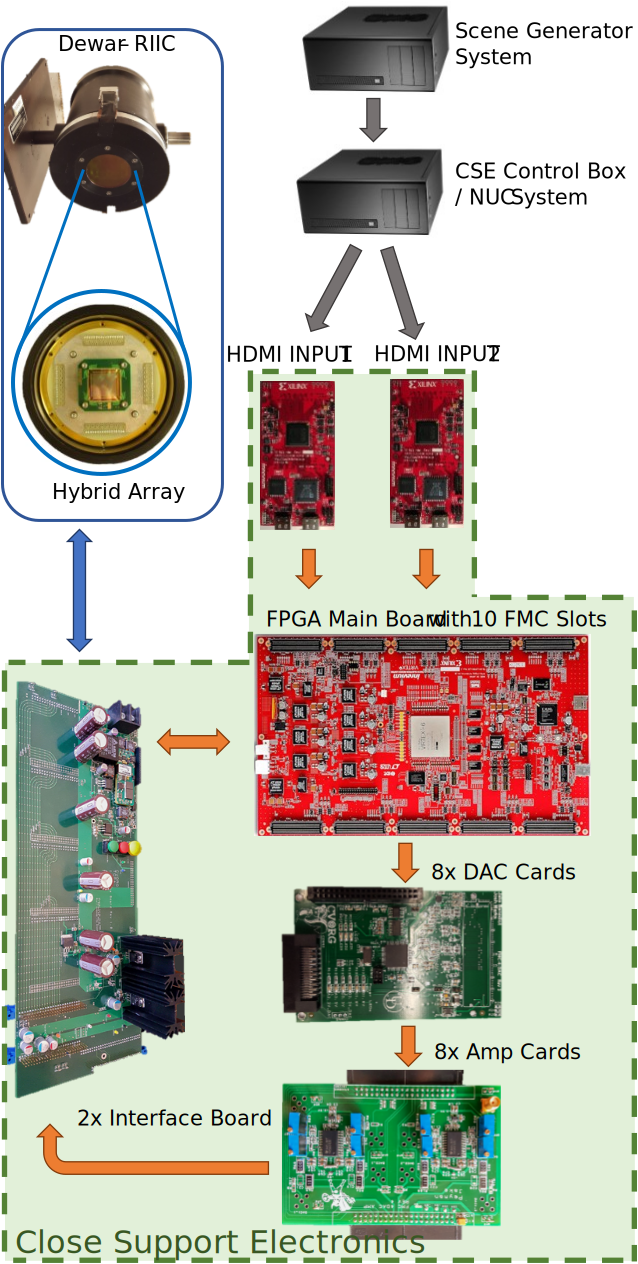
\includegraphics[width=0.65\textwidth]{fig/sleds_block.pdf}
        \caption{SLEDS System Block Diagram}
        \label{fig:sleds_block}
    \end{figure}

    Once enough data is buffered, the firmware will control the write process to drive the 8 DAC cards which each house 2 16-bit DAC integrated circuits per card, with each circuit consisting of 2 channels per DAC. Yielding 32 parallel channels with 512 total signals. Once the DAC process is done, the analog output of the 32 channels is then amplified and routed to the array through ribbon cables. Figure~\ref{fig:nessie_enclosure_internals} shows the components installed within a CSE with the ribbon cables shown in the top right. Additional control signals provided by the firmware and routed to the RIIC through these cables are discussed in Chapter~\ref{sec:array_Interleaved_write_process}. The specifics of the PDP firmware architectures write process are discussed in Chapter~\ref{chap:implementation}.

    \begin{figure}
        \centering
        \includegraphics[width=1.0\textwidth]{fig/nessie_enclosure_internals.jpg}
        \caption{CSE Internals}
        \label{fig:nessie_enclosure_internals}
    \end{figure}

    Figure~\ref{fig:cse_comm_block} shows the internals of CSE communication. Communication for controlling the behavior of CSE is done through a daisy chained set of UART devices utilizing a reliable two way communication protocol called the CVORG protocol\footnote{Named after my research group at the University of Delaware.}. Without loss of generality, the protocol itself consist of commands to control various aspects of operation, such as, tripping an array, setting voltage limits, and configuring firmware operation. It also allows for information to be retrieved about current system configuration, as well as, operational errors. The destination of an operation is encoded as part of each command. Thus, commands not meant for a given component are forwarded along the chain. Memory mapped I/O between the frontend and backend firmware is controlled by the microblaze soft processor and used to control the underlying PDP firmware registers, as well as, program an array using Serial Peripheral Interface (SPI) (Not shown). The underlying details of the CVORG protocol itself are beyond the scope of this work and will not be discussed here. The details of command operations will be discussed in Chapter~\ref{sec:frontend_arch}. Additionally, SPI communication is also used to send data for LCD readout. Typically this includes voltage and current information, as well as, the results of power on sanity checks. Finally, the details of the processing performed on HDMI display data sent directly to the Backend Firmware as will be discussed in Chapter~\ref{sec:backend_arch}.

    \begin{figure}
        \centering
        \includegraphics[width=1.0\textwidth]{fig/cse_comm_block.pdf}
        \caption{CSE Internal Communication Block Diagram}
        \label{fig:cse_comm_block}
    \end{figure}

    Figures~\ref{fig:external_cse_comm_direct},~\ref{fig:external_cse_comm_half_indirect},~and~\ref{fig:external_cse_comm_indirect} show the details of external communication to a CSE in various configurations. In all configurations, a Low Pin Count (LPC) FPGA Mezzanine Card (FMC) connector provides the ability for various interfaces to be used to send data to the CSE, such as serial protocols or display based protocols over different types of hardware links. The FMC interface cards are responsible for retrieving the data over the link and formatting it in a manner that the internal CSE FPGA can decode. In practice, 24-bit pixel words and a data enable pin are utilized. In display protocol setups, a vertical sync signal is also utilized to reset pixels every display frame. As mentioned earlier in this section, current CSE setups utilize two HDMI FMC cards for input where the input for the top half of an array will be delivered over one cable and the bottom over the other. API communication on the other hand utilizes UART and the CVORG protocol.

    \begin{figure}
        \centering
        \includegraphics[width=1.0\textwidth]{fig/external_cse_comm_direct.pdf}
        \caption{CSE External Direct Communication Block Diagram}
        \label{fig:external_cse_comm_direct}
    \end{figure}

    Figure~\ref{fig:external_cse_comm_direct} depicts direct communication in which formated scene data is sent directly to a CSE and system configuration is done directly by a scene generator. In this type of setup, the scene generator can monitor CSE operation directly, as well as, operate in either a closed or open loop type setup. This type of setup is desirable for minimizing end-to-end latency within an system for use cases where performance is paramount. For example, closed loop scenerios may feed recorded output imagery from an array back into the scene generator for in the loop analysis or in some cases subsequent frames may depend on the recorded results from prior frames.

    \begin{figure}
        \centering
        \includegraphics[width=1.0\textwidth]{fig/external_cse_comm_half_indirect.pdf}
        \caption{CSE External Indirect API Communication Block Diagram}
        \label{fig:external_cse_comm_half_indirect}
    \end{figure}

    Figure~\ref{fig:external_cse_comm_half_indirect} depicts indirect API communication in which system configuration is done through client APIs, and scene data is sent directly to a CSE. This type of setup is useful for situations where control over a CSE is needed but where API operation cannot be tightly coupled with a scene generator due to development costs, practical reasons, etc. In this setup, thin client API shims are provided to execute commands using remote procedure calls (RPC) which then are executed within a CSE operations box to communicate with the CSE. Similar to the direct setup, end-to-end latency is minimized by directly driving an array.

    \begin{figure}
        \centering
        \includegraphics[width=1.0\textwidth]{fig/external_cse_comm_indirect.pdf}
        \caption{CSE External Indirect API and Data Communication Block Diagram}
        \label{fig:external_cse_comm_indirect}
    \end{figure}

    Figure~\ref{fig:external_cse_comm_indirect} depicts an indirect setup in which both API communication and scene data are sent to an intermediate CSE operations box. This type of setup is utilized in the event that data cannot be formatted directly for display on an array within a scene generator. It may also be utilized in cases where non-uniformity correction is performed externally from scene generation as shown in Figure~\ref{fig:sleds_block}. A third scenerio where this type of setup may be used is without a scene generator, where a CSE operation box could be used to characterize an array directly, as well as, to test and troubleshoot operations. Similarly, to the other indirect API communication setups, client API shims are provided to execute commands using remote procedure calls (RPC) which then are executed within a CSE operations box to communicate with the CSE.

\section{Array Interleaved Write Process}
    \label{sec:array_Interleaved_write_process}
    As will be discussed in Chapter~\ref{sec:classical_display_protocols}, while all current IRSP arrays utilize some display protocol technology that is decoded in order to drive an array's pixels, arrays may utilize different internal drawing mechanisms for driving the pixels. This section discusses the details of those mechanisms within the TCSA, NSLEDS, and HDILED arrays for conceptual purposes, and while the details may differ for other arrays, the overall raster write process is generalizable in the sense that not all pixels will be driven at once but some subset. Even arrays which operate in a snapshot mode where all pixels turn on at the same time will charge subsets of pixels over some time frame and enable the pixels only once all are charged. The write order and number of pixels driven at the same time would be array dependent though.

    %FIXME: add proper citation for Tianne paper when published
    The TCSA, NSLEDS, and HDILED arrays are organized into four quadrants as shown in Figure~\ref{fig:tcsa_nsleds_hdiled_quads}. Each quadrant is organized into a given number of pixels with TCSA housing 256 by 256, NSLEDS housing 512 by 512, and HDILED housing 1024 by 1024 per quadrant. There are number of input signals necessary to drive an array. These are {\em a 4 bit quadrant write enable}, {\em X address}, {\em Y address}, {\em LOAD bit}, {\em 16 Strong/Weak drive strength bit}, {\em array reset bit}, and {\em analog signaling lines which charges the pixels being addressed}. The quadrant write enable, X address, Y address, and LOAD signals are all utilized for addressing the array.

    \begin{figure}
        \centering
        %includegraphs[trim=L B R T]
        \includegraphics[width=1.0\textwidth]{fig/tcsa_nsleds_hdiled_quads.pdf}
        \caption[TCSA, NSLEDS, and HIDLED Array Quadrant Layouts]{TCSA, NSLEDS, and HIDLED Array Quadrant Layouts\textsuperscript{a}}
        \vspace{-8px}
        \footnotesize\textsuperscript{a} Not drawn to scale
        \label{fig:tcsa_nsleds_hdiled_quads}
    \end{figure}

    The quadrant write enable selects which quadrant to drive. It is worth noting that each quadrant has separate internal signaling which allows for each quadrant to operate independently in parallel when mounted in a package that provides independent external signals. However, to date most of the fabricated IRLED arrays are mounted in packages that allows for only one quadrant to be drawn at a time\footnote{Currently, only HIDLED has been tested in the type of setup\cite{lassiter1, LassiterEtAl2019_1, LassiterEtAl2019_2, lassiter3} due to it having the largest resolution per quadrant.}. In a setup being driven in parallel, multiple CSEs are utilized. In a two CSE setup, half of the quadrant bits would be controlled by one CSE and half by another. In a four CSE setup, a single quadrant would be controlled by a single CSE. Irrespective of the number of CSEs used to a drive an array, the internal RIIC signal lines would be driven in precisely the same manner within each quadrant with the only change being that they operate asynchronously with respect to the others.

    The X address, Y address, and LOAD are used to select which pixel or group of pixels to write within a quadrant depending on the mode of operation. Though these lines are effectively shared by quadrants in a single CSE Setup, within the RIIC architecture they can be driven independently for each quadrant. Internally, each array can write up to 32 pixels (or channels) of data at a given time. The mode of operation dictates whether 2, 4, 8, 16, or 32 channels are used. The number of address bits utilized depends on the mode of operation. The amount of address bits differs by array due to the differences in sizes. NSLEDS utilizes 7 bits for the X address and 7 bits for the Y address, yielding a total of 256 by 256 addresses per quadrant. The LOAD bit is used to select between even and odd rows, yielding an effective address space of 256 by 512 per quadrant. Because the smallest mode of operation writes 2 pixels at a time, this is sufficient to fully address the array. Similarly, HDILED utilizes 8 bits for the X address and 8 bits for the Y address, yielding a total of 512 by 512 addresses per quadrant. Again, as with NSLEDS, the LOAD bit is used to select between even and odd rows, yielding an effective address space of 512 by 1024 per quadrant. This is again sufficient to completely address the array since it also can at a minimize write 2 pixels at a time.

    Structurally, NSLEDS and HIDLED are layed out as super pixel as shown in Figure~\ref{fig:nsleds_hdiled_array_superpixel_layout}. Each super pixel is made up of a grid of 4 pixels spanning two rows and columns. These are layed out across the array in a grid structure with NSLEDS consisting of 256 by 256 super pixels, and HIDLED consisting of 512 by 512 super pixels. This image also highlights two points discussed above, the LOAD line selects between the top two pixels (even rows) and bottom two pixels (odd rows) of each super pixel in the quadrant, and the two selected pixels are both written at the same time. Additionally, these share a drive strength as noted in the diagram. This is controlled using the Strong/Weak drive strength bits which dictate whether to provide a strong or weaker light emission for the given pair of pixels.

    \begin{figure}
        \centering
        %includegraphs[trim=L B R T]
        \includegraphics[width=0.70\textwidth]{fig/superpixel_layout.pdf}
        \caption{NSLEDS/HDILED Array Super Pixel Layout}
        \label{fig:nsleds_hdiled_array_superpixel_layout}
    \end{figure}

    The 32 analog signaling lines control the emission intensity of driven pixels. These 32 channels are controlled by digital to analog converters within the CSE that are driven by the firmware. Internally, a CSE has 8 DAC cards with 2 DAC integrated circuits per card, with each DAC circuit consisting of 2 DAC channels as discussed in Chapter~\ref{sec:close_support_electronics}. Each channel is used to drive a single pixel, giving the ability to drive 32 pixels at once or some subset as mentioned previously.

    In practice, it is perferable to utilize all channels at once because this allows for more pixels to be driven in a shorter amount of time. Figure~\ref{fig:nsleds_hdiled_array_interleaved_pixel_mapping_per_write} shows the pixel mapping per write for 32 physical pixels on an array. 2 by 32 columns of pixels are shown segmented into super pixels. The Y address denotes the 16 super pixels that are selected per address. If Y is incremented by 1 then the next 16 rows of super pixels would be selected. X address (not shown) simply selects the next two columns of super pixels. DAC Card denotes which DAC card drives the given super pixel. L denotes which value of LOAD will select which columns within super pixels. When LOAD is low as shown in the middle segment, the top super pixels are selected as indicated in cyan. When LOAD is high as shown in the right segment, the bottom super pixels are selected.

    \begin{figure}
        \centering
        \includegraphics[width=0.95\textwidth]{fig/nsleds_hdiled_array_writing.pdf}
        \caption{NSLEDS/HDILED Array Interleaved Pixel Mapping Per Write}
        \label{fig:nsleds_hdiled_array_interleaved_pixel_mapping_per_write}
    \end{figure}

    The overall writing process for writing 64 pixels is a two step process. First, 32 values for the even rows are loaded in and written to the array, followed by 32 values from the odd rows being loaded and written to the array. At a data level, it is ideal to interleave the data such that it is avaliable at the optimal time in order to reduce latency and buffering requirements within the firmware. This is discussed in detail in Chapter~\ref{chap:pdp_protocol}.

    Writing additional segments of pixels largely means buffering more data and repeating the same write process while asserting the correct address lines. Given that the arrays have no inherit hardware required write order other than what has been discussed above, the exact order of writing independent segments of 32 pixels can change depending on a number of factors. In a single CSE Setup, under most circumstances, the data for the top quadrants is carried by a single HDMI input going into a CSE, and the data for the bottom quadrants carried by the other HDMI input\footnote{When utilizing PDP for driving an array the location of where data is to be written on an array is agnostic to the HDMI input the data is carried on.}. In this case, the CSE firmware will swap between writing segments of 32 or 64 pixels to the top and bottom halves of an array. The former if it is desirable to write a minimal amount of data before servicing data from another input, the latter if it is desirable to complete an entire chunk of pixels. In a two CSE Setup, data over the hdmi links data could be segmented either horizontally or vertically meaning that each HDMI link would carry an entire quadrants data. In a four CSE setup, each link would carry half a quadrants data. As the reader may imagine, the order of writes could be configured in many different ways under these scenerios. Though it will not be discussed in detail within this thesis, it is worth noting for posterity that the order of writes on IRLED arrays does affect the thermal load on an array which has an effect on pixel brightness\cite{BarakhshanEtAl2017, LaVeigneSieglinger2012, norton2}; thus, controlling the order of writes can be an important factor to consider for designers and users of a system.

    %FIXME: Add details about delays into the RIIC and aligning signals maybe?
    %FIXME: slow channels
\section{Data ordering}
    Due to the interleaved write process described in Chapter~\ref{sec:array_Interleaved_write_process}, data sent to an array is reordered in a manner that simplifies firmware development and minimizes buffering requirements. Figure~\ref{fig:bit_packing} shows the data bitpacking utilized within the system. It's designed to map to the superpixel layout shown in Figure~\ref{fig:nsleds_hdiled_array_superpixel_layout}. Shown is a 24-bit pixel word which normally represents an RGB value in RGB color space within display protocols where 8 bits are reserved for each of the red, green, and blue channels. Below this is the mapping of each bit value for an NSLEDS or HDILED array. Where \textbf{S} indicates the drive strength of the super pixel, \textbf{L} indicates the value to drive the left side of the super superpixel at, and \textbf{R} indicates the value to drive the right side of the superpixel at. Only 11 bits are currently used to transmit data per pixel due to bit resolution limitations in the DAC and amplifier boards used within a CSE\footnote{Future CSEs may have higher bit resolutions resulting in the need for 16-bits per pixel to be transmitted. In this event bitpacking would not be used}.

    \begin{figure}
        \centering
        \includegraphics[width=1.0\textwidth]{fig/bit_packing.pdf}
        \caption{Bit-packing Format}
        \label{fig:bit_packing}
    \end{figure}

    Figure~\ref{fig:image_encoding} shows the input reordering needed to be done for data sent to a CSE. Each cable sends half of the data as noted in Chapter~\ref{sec:close_support_electronics}. The input example is segmented into top, middle, and bottom to indicate which part goes over which input and the different reordering steps. The portions denoted as \textbf{Top} are transmitted over CSE input 1. The portions denoted as \textbf{Bottom} are transmitted over CSE input 2. The portions marked \textbf{Middle} are split evenly over both inputs evenly. The first step of data reordering is to bitpack into 11-bit words as shown in Figure~\ref{fig:bit_packing}. Next, even/odd reordering is performed to reduce latency and buffering constraints as will be shown in more detail in subsequent figures. Finally, data is transposed before being sent to the array in order to accommodate the column write order of the array shown in Figure~\ref{fig:nsleds_hdiled_array_interleaved_pixel_mapping_per_write}. If data was not transposed in this manner, then multiple lines of data would need to be buffered in order to draw 32 pixels for a single write\footnote{Earlier pre-pdp firmware implementations required full image buffering before displaying a single pixel on an array resulting in an entire frame of latency}. It is worth noting that as mentioned in Chapter~\ref{sec:array_Interleaved_write_process}, different arrays could have different rasterization processess, and in that event the transformations described here would need to be changed to minimize buffering for those scenerios.


    \begin{figure}
        \centering
        \includegraphics[width=1.0\textwidth]{fig/image_encoding.pdf}
        \caption{Image Encoding: Input Reordering}
        \label{fig:image_encoding}
    \end{figure}

    Figure~\ref{fig:image_encoding_quads} shows how the same image data maps to each quadrant on an array. Similarly, to the previous image the separation of top, middle, and bottom by input cable holds here. Additionally, shown is that quadrant one and two are transmitted over the first input and quadrant three and four over the second input. Note also, that the top-left of the image corresponds to quadrant one, the top-right of the image corresponds to quadrant two, the bottom-left of the image corresponds to quadrant three, and the bottom-right of the image corresponds to quadrant four. This relationship holds for all subsequent images. Figure~\ref{fig:image_encoding_colored} shows the same details in a colored chart.

    \begin{figure}
        \centering
        \includegraphics[width=1.0\textwidth]{fig/image_encoding_quads.pdf}
        \caption{Image Encoding: Quadrant Reordering}
        \label{fig:image_encoding_quads}
    \end{figure}

    \begin{figure}
        \centering
        \includegraphics[width=1.0\textwidth]{fig/image_encoding_colored.pdf}
        \caption{Image Encoding: Quadrant Reordering with Color Overlay}
        \label{fig:image_encoding_colored}
    \end{figure}

    Figure~\ref{fig:image_encoding_bitback} shows the bit-packing process for a false color image in order to aid with understanding. The blown up sections show single columns of data and the cooresponding bitpacked version of the data where two columns of input with different colors of data per column are merged into a single column of 24-bit data with one color. This results in the example input image having two solid colors after bit-packing. In the actual implementation of bitpacking, real data is in the IR-spectrum and not averaged in this way, but clamped and scaled instead. While not required, generally IR data is normally 16-bits per pixel which corresponds to current higher class IR detectors having a dynamic range of 14 per pixel\cite{FLIR1, FLIR2, FLIR3}. Cheaper detectors may only have lower dynamic ranges resulting in a lower ability to differentiate light output.

    \begin{figure}
        \centering
        \includegraphics[width=1.0\textwidth]{fig/image_encoding_bitback.pdf}
        \caption{Image Encoding: Data Bitpack}
        \label{fig:image_encoding_bitback}
    \end{figure}

    Figure~\ref{fig:image_encoding_bitpack_reorder} shows a false color input image designed to highlight the data reordering applied to imagery. The blown up sections show 64 labeled rows of input data where the even rows are one color and the odd rows another for ever 32 rows. For every 32 rows, the even and odd rows are de-interlaced into 16 even rows of data follow by 16 odd rows of data. In the example input image this results in every 16 de-interlaced rows to have have a different color. This is due to the interleaved writing processing for individual 32 pixel writes discussed in Chapter~\ref{sec:array_Interleaved_write_process}. Reordering data in this manner allows for only 16 pixels of data (or 32 in terms of bitpacking) to be buffered per write. Without the is reordering, double the amount of pixels would need to be buffered per array write increasing both latency and implementation complexity.

    \begin{figure}[H]
        \centering
        \includegraphics[width=1.0\textwidth]{fig/image_encoding_reorder.pdf}
        \caption{Image Encoding: Data Reorder}
        \label{fig:image_encoding_bitpack_reorder}
    \end{figure}

    Figures~\ref{fig:image_encoding_color_example1},~\ref{fig:image_encoding_color_example2},~and~\ref{fig:image_encoding_color_example3} show some examples of what false colored images would look like if processed by the reordering kernels in order to give the reader a better understanding of how different types of data would look when during the intermediate processes. Note the charateristic jagged pattern due to even/odd row reordering present in each image.

    \begin{figure}[H]
        \centering
        \includegraphics[trim=0 40pt 0 40pt,width=0.90\textwidth]{fig/image_encoding_pac.pdf}
        \caption{Image Encoding: Color Example 1}
        \label{fig:image_encoding_color_example1}
    \end{figure}

    \begin{figure}[H]
        \centering
        \includegraphics[trim=0 40pt 0 40pt,width=0.90\textwidth]{fig/image_encoding_liberty.pdf}
        \caption{Image Encoding: Color Example 2}
        \label{fig:image_encoding_color_example2}
    \end{figure}

    \begin{figure}[H]
        \centering
        %includegraphs[trim=L B R T]
        \includegraphics[trim=0 40pt 0 40pt,width=0.90\textwidth]{fig/image_encoding_origami.pdf}
        \caption{Image Encoding: Color Example 3}
        \label{fig:image_encoding_color_example3}
    \end{figure}

    Figures~\ref{fig:image_encoding_ir_example1},~and~\ref{fig:image_encoding_ir_example2} show IR imagery going through the process of reordering. The image shown in Figure~\ref{fig:image_encoding_ir_example1} is commonly used to focus IR cameras and for testing IR array behavior with various shapes and numbers. The image shown in Figure~\ref{fig:image_encoding_ir_example2} is test imagery from one of my labs projects.

    \begin{figure}[H]
        \centering
        %includegraphs[trim=L B R T]
        \includegraphics[trim=0 40pt 0 0,width=1.0\textwidth]{fig/image_encoding_ir1.pdf}
        \caption{Image Encoding: IR Example 1}
        \label{fig:image_encoding_ir_example1}
    \end{figure}

    \begin{figure}[H]
        \centering
        %includegraphs[trim=L B R T]
        \includegraphics[trim=0 40pt 0 40pt,width=1.0\textwidth]{fig/image_encoding_ir2.pdf}
        \caption{Image Encoding: IR Example 2}
        \label{fig:image_encoding_ir_example2}
    \end{figure}

    \chapter{Display Protocols} % DONE
        This chapter discusses the details of display protocols. Firstly, it provides a general discussion of how common display protocols work to send pixel data to a display system (e.g. a television). Then, it discusses how these protocols are utilized within IRSP technology.

\section{Classical Display Protocols}
    \label{sec:classical_display_protocols}

    Display specifications such as DSI\cite{HDMIForum2017}, DVI\cite{DDWG1999}, HDMI\cite{HDMIForum2018}, and DisplayPort\cite{VESA2016} are the backbone of consumer electronic display devices. They are utilized in a plethora of devices ranging from televisions, monitors, laptops, smart phones, to embedded devices such as point of sale (POS) terminals. Increasingly, they are being utilized in the ever increasing smart display market for applications such as registration, product menus, smart watches, etc.

    These generally provide a standardized feature-set, or display protocol, that is rooted in classical analog video specifications (e.g. VGA, Composite)\cite{NIAnalog} that utilize scan lines\cite{Neal1998}. Scan lines are used to provide video timing information in order to synchronize a display to a given refresh rate. Each scan line consist of an active video region followed by a horizontal blanking period. After all active video scan lines are displayed, a vertical synchronization region is used to indicate the end of a frame.

    %FIXME add crosssectional blowout chart

    An overview of this is shown in Figure~\ref{fig:display_protocol_timing_overview}. The region shown in green is the pixel data for the active video region of the display. It is of size $H_a\times V_a$ which represents the number of pixels to display, for example, 1920 by 1080 for a HDTV high-definition video mode\cite{MythTVWebsite}. The blanking time regions denote pixel data that is sent but not displayed\footnote{Typically data lines are held low during this period, but somtimes it is used for out-of-band communication to send other information such as audio encoding.}. A scan line consist of pixels made up of $h_a$, the horizontal active size; $h_{fp}$, the horizontal front porch before the pulse signal; $h_{sp}$, the horizontal sync pulse; and $h_{bp}$, the horizontal back porch after the sync pulse. The vertical blanking period makes up multiple scanlines and consist of $v_{fp}$, the vertical front porch before the vsync pulse; $v_{sp}$, the vertical sync pulse; $v_{bp}$, the vertical back porch after the vertical sync pulse. Sync pulses are generally active low, meaning that during active display a sync signal is high as shown in the diagram.

    \begin{figure}
        \centering
        \includegraphics[width=1.0\textwidth]{fig/display_timing_overview.pdf}
        \caption{Display Protocol Timing Overview}
        \label{fig:display_protocol_timing_overview}
    \end{figure}

    Figure~\ref{fig:display_protocol_line_cross} shows a closeup view of signal lines during the active region of display for two scan lines. A data enable signal denoted by $enable$ is high during the active region shown in green. Following this, it goes low for a period of time denoted by $h_{fp}+h_{sp}+h_{bp}$. The horizontal sync signal goes low only in the region shown in yellow between the front porch and back porches. This process repeats for all scan lines. Once the last active region pixel is drawn, the enable signal will stop going high during the vertical synchronization period.

    \begin{figure}
        \centering
        \includegraphics[width=1.0\textwidth]{fig/display_timing_line_cross.pdf}
        \caption{Display Protocol Horizontal Signal Cross Section Timing}
        \label{fig:display_protocol_line_cross}
    \end{figure}

    %FIXME: Fix discussion of DP not using fucking backwards compatibility shitty hdmi fucking mode
    %FIXME: Talk about CC in the vertical blanking

    Figure~\ref{fig:display_protocol_full_cross} shows a closeup view of signal lines during the transition into the vertical synchronization period. The region donated by $V_a$ indicates the end of the video active region of the display which occurs toward the end of a frame. After the active video region, all data has been drawn to a display. The region denoted by $v_{fp}+v_{sp}+v_{bp}$ is the vertical blanking or vsync period during which no active video data is sent; therefore, data enable denoted by $enable$ is always low during this period. Before the vertical sync pulse period denoted by $v_{sp}$ occurs, a vertical front porch period denoted by $v_{fp}$ occurs. After the vertical sync pulse, a vertical back porch region $v_{bp}$ occurs. Following this the beginning of the next frame occurs as denoted by $v_{a+1}$.

    \begin{figure}
        \centering
        \includegraphics[width=1.0\textwidth]{fig/display_timing_full_cross.pdf}
        \caption{Display Protocol Full Signal Cross Section Timing}
        \label{fig:display_protocol_full_cross}
    \end{figure}

    Figure~\ref{fig:modeline_refresh_rate} shows the relationship between between the different regions of a display and the frequency or refresh rate. $l_h$ denotes the scan line size of a display, or total horizontal width, which is made up of the horizontal active and horizontal porch region pixels of a display. $l_v$ denotes the total vertical width of a display, which is made up the vertical active and vertical porch region pixels of a display. Each pixel is sent at a rate denoted by $f_p$, the pixel frequency (also called the pixel clock). $f_f$ denotes the frame frequency or frame rate of a display. This is simply the pixel frequency over the total number of pixels (video active and porches) of a display. $p_t$ denotes the time period a single pixel takes to send. $f_t$ denotes the time period for an entire frame.

    \begin{figure}
        \centering
        { \Large
            $l_h=h_a+h_{fp}+h_{sp}+h_{bp}$ \vspace{8px} \\
            $l_v=v_a+v_{fp}+v_{sp}+v_{bp}$ \vspace{8px} \\
            $f_f={\frac{f_p}{l_h \cdot l_v}}$ \\
            $p_t={\frac{1}{f_p}}$ \vspace{8px} \\
            $f_t={\frac{1}{f_f}}$ \vspace{8px}
        }
        \caption{Total Refresh Rate}
        \label{fig:modeline_refresh_rate}
    \end{figure}

    %FIXME: example modeline
    To illustrate, let us look at the display modeline generated using the VESA Coordinated Video Timing (CVT) standard shown in Figure~\ref{fig:modeline_example}. This modeline operates a total frame frequency of approximately \mbox{30 Hz}. The pixel clock 79.75, denoted in red, is specified in megahertz. The horizontal pixels, denoted in blue; are the end of horizontal active, the end of horizontal front porch, the end of horizontal sync pulse, and the end of horizontal back porch respectively. The vertical pixels (measured in lines), denoted in green; are the end of vertical active, the end of vertical front porch, the end of vertical sync pulse, and the end of horizontal back porch respectively. The sync pulse polarities, denoted in yellow; indicate whether a given sync pulse is active low or active high. A minus symbol indicates active low and a plus symbol indicates active high. If these numbers are placed into into the formulas shown in Figure~\ref{fig:modeline_refresh_rate} the results shown in Figure~\ref{fig:modeline_refresh_rate_plug} are yielded. The astute reader will note that $l_h$ and $l_v$ are the same as the total pixel size for the given modeline. The pixel period is $\sim12.53 ns$, meaning that each pixel is drawn for the given amount of time. The frame period is $\sim33.33 ms$, meaning that each frame is drawn for that given amount of time.

    \begin{figure}
        \centering
        { \normalsize
        \textbf{``1920x1080\_30.00"} {\color{red}79.75}  {\color{blue} 1920 1976 2168 2416}  {\color{darkgreen}1080 1083 1088 1102} {\color{olive}-hsync +vsync}
        %\vspace{-8px}
        }
        \caption{VESA CVT Generated Modeline}
        \label{fig:modeline_example}
    \end{figure}

    %FIXME: finish this chart
    \begin{figure}
        \centering
        { \Large
            $h_a=1920; h_{fp}=1976-h_a; h_{sp}=2168-h_{fp}; h_{bp}=2416-h_{sp};$ \\
            $v_a=1080; v_{fp}=1083-v_a; v_{sp}=1088-v_{fp}; v_{bp}=1102-v_{sp};$ \\
            $l_h=2416=1920+56+192+248$ \vspace{8px} \\
            $l_v=1102=1080+3+5+14$ \vspace{8px} \\
            $f_p=79.75e6$ \vspace{8px} \\
            $f_f=30.0={\frac{f_p}{l_s \cdot l_c}}$ \\
            $p_t=12.53ns={\frac{1}{f_p}}$ \vspace{8px} \\
            $f_t=33.33ms={\frac{1}{f_f}}$ \vspace{8px}
        }
        \caption{Computed Refresh Rate for a 30Hz CVT Modeline}
        \label{fig:modeline_refresh_rate_plug}
    \end{figure}

    Chapter~\ref{sec:displays_within_proj_system}, discusses how these protocols are utilized within an IRLED projector system, briefly highlight the limitations, and . %FIXME: finish this paragraph

\section{Display Protocols within IRSP Technology}
    \label{sec:displays_within_proj_system}
    % Finally, it discusses how these protocols are utilized within an IRLED project system.
    IRSP technology typically utilizes classical display protocol technology in some form in order to drive IR-arrays. In the most basic form a scene generator will provide imagery that is encoded utilizing one of the protocols discussed and send it to some form of CSE which will then simply decode it.

    For scenerios that involve unsynchronized operation where dropped frames are not an issue, these protocols can largely be used without modification. However, scenerios that require synchronization in either open loop or closed loop setups present a challenge. Often, non-standard modifications must be used to compensate for jitter among different system processes and overall system latency. This can range from utilizing off the shelf components such as Nvidia Quadro Sync cards\cite{NVIDIAQuadroSync} or developing additional hardware pipelines capable of buffering and delaying emission of frame data. This presents a particular challenge because the user typically does not have direct control over frame buffers, frame emission, or the software drivers within a system. Moreover, encoders and decoders expect the protocols to work in a defined way that modifications could run afoul of.

    \chapter{Packetized Display Protocol}
        \label{chap:pdp_protocol}

This chapter discusses the underlying communication details of the packetized display protocol (PDP) architecture. First, it gives an overview of the protocol design methodology. Followed by a discussion of the generalized packet format. Finally, it discusses individual packet types. The central purpose of this chapter is to provide the reader with an understanding of the reasoning behind design decisions, as well as, to provide a detailed specification of the protocol.

\section{Design Methodology}
    The design methodology for the PDP protocol began with a number of critical design goals. The first goal was to design a scalable display system that was distributable and hardware agnostic. The second design goal was to provide a protocol that was relatively simple to implement without unnecessary complexity to ease the encoding and decoding process. A low overhead and fast decode process is crucial to ensuring latency is sub-frame\footnote{This refers to latency of that below the time it would take to buffer an entire frame. Which is a common synchronization method utilized in projector systems.} across the system. Additionally, simplifying these processes also eases potential hardware implementation mistakes, as well as, inefficiencies that could lead to reduced performance. The third goal was to provide dynamic intra-frame variable refresh rate (VRR) to enable better bandwidth utilization. In particular, to allow for regions of a display to be intelligently updated at different rates when driven by a scene generator. The fourth goal was to provide a path to utilize classical display protocol streams such as HDMI with PDP without introducing overhead. This is to allow for interoperability where necessary when utilizing classical display sources, and to ease migration to a PDP based system.

    \subsection{Comparison to Classical Display Protocols}
        In order to better understand how to design PDP, the constraints of classical display protocols were investigated to discern which features within these protocols conflict with the design goals of PDP. In addition, it was necessary to investigate whether these could provide a path forward in the design and development of PDP. Many versions of these protocols (DVI\cite{DDWG1999}, HDMI\cite{HDMIForum2018}, DisplayPort\cite{VESA2016}, etc.) provide similar feature-sets to end-users with the major focus being on increasing refresh rates and resolutions with each new specification. However, as discussed in Chapter~\ref{sec:classical_display_protocols}, their basis is rooted in the classical analog video specifications that utilize scan lines\cite{Neal1998}. This means, that signal timing utilizes vertical and horizontal blanking periods that consist of a front-porch, sync pulse, and back-porch; in addition to, the active video data to be displayed.

        For early analog display devices, these signals enabled operators to manually adjust horizontal and vertical hold times relative to the sync pulses in order to correct for the imprecise timing of early display hardware; but provide little benefit on modern hardware other than as an embedded method to support sending frames at a static interval, and to enable tearless buffer swapping in either double buffering\cite{FriedbergEtAl1990} or triple buffering schemes\cite{3dfx1997} utilized within GPUs\footnote{This is performed by swapping buffers during the vertical sync (vsync) interval of a frame\cite{3dfx1999,3dfx1999_2}. See Chapter~\ref{chap:display_protocols} for details about the vsync interval.}. In digital display technology, this represents an anachronism that impedes the goal of maximizing bandwidth utilization when driving a display by requiring the transmission of unnecessary data over the digital protocol. For example, a commonly utilized 1920 by 1080 pixel mode operating at \mbox{60 Hz}\cite{MythTVWebsite} on a modern display has a 16 percent blanking period overhead due to the specification of vertical and horizontal sync periods. Other examples can be seen in Table~\ref{tbl:modeline_overhead}. Of note, the smaller resolutions were tested on existing hardware in order to minimize the overhead in blanking. What one sees is that as modelines shrink and data rates decrease higher percentages of blanking is required relative to displayed pixels. This is due to the inability for common implementations of video decoders to operate correctly when blanking is minimized and in many cases simply at all when non-standard resolutions are utilized.

        \begin{table}
            \centering
            \large
            \begin{tcolorbox}[tabularx={Y|Y|Y|Y|Y},title=\textbf{Modeline Overhead},boxrule=0.5pt]
            \textbf{Resolution} & \textbf{Refresh Rate (Hz)} & \textbf{Visible Pixels} & \textbf{Total Pixels} & \textbf{Overhead} \\ \hline
                \textbf{1920x1080} & \textbf{60}   & 2073600 & 2475000 & 16.2\% \\ \hline
                \textbf{1600x1200} & \textbf{60}   & 1920000 & 2700000 & 28.9\% \\ \hline
                \textbf{1280x1024} & \textbf{60}   & 1310720 & 1799408 & 27.2\% \\ \hline
                \textbf{1280x960}  & \textbf{60}   & 1228800 & 1800000 & 31.7\% \\ \hline
                \textbf{1280x800}  & \textbf{60}   & 1024000 & 1391040 & 26.4\% \\ \hline
                \textbf{1024x768}  & \textbf{60}   & 786432  & 1083264 & 27.4\% \\ \hline
                \textbf{500x500}   & \textbf{500}  & 250000  & 296100  & 15.6\% \\ \hline
                \textbf{500x500}   & \textbf{400}  & 250000  & 296100  & 15.6\% \\ \hline
                \textbf{500x500}   & \textbf{300}  & 250000  & 357500  & 30.1\% \\ \hline
                \textbf{500x500}   & \textbf{100}  & 250000  & 357500  & 30.1\% \\ \hline
                \textbf{500x500}   & \textbf{60}   & 250000  & 357500  & 30.1\% \\ \hline
                \textbf{500x500}   & \textbf{50}   & 250000  & 364000  & 31.3\% \\ \hline
                \textbf{500x500}   & \textbf{30}   & 250000  & 520000  & 51.9\% \\ \hline
                \textbf{500x500}   & \textbf{30}   & 250000  & 520000  & 51.9\% \\ \hline
                \textbf{500x256}   & \textbf{1000} & 131072  & 149460  & 12.3\% \\ \hline
                \textbf{500x256}   & \textbf{500}  & 131072  & 256000  & 48.8\% \\ \hline
                \textbf{500x256}   & \textbf{200}  & 131072  & 320000  & 51.9\% \\ \hline
                \textbf{500x256}   & \textbf{100}  & 131072  & 320000  & 59.0\% \\ \hline
                \textbf{500x256}   & \textbf{60}   & 131072  & 320000  & 59.0\% \\ \hline
            \end{tcolorbox}
            \caption[Modeline Overhead]{Modeline overhead for various resolutions and refresh rates\cite{MythTVWebsite}. Computed using active pixel area over total pixel area. 500x500 and 512x256 are typical modeline resolutions used on IRLED arrays.}
            \label{tbl:modeline_overhead}
        \end{table}

        These protocols also internally utilize a mode based display of data that requires the specification of the absolute width and height of display, as well as, a pixel clock which when used in conjunction with the vertical blanking information provides a total refresh rate as described in Chapter~\ref{sec:classical_display_protocols}. This means that the bandwidth requirements for a given mode are inherently static across all frames. In addition, this constrains the refresh rate for a display to be static in terms of both the intra-frame regions of the display and between frames. Effectively increasing the burden of synchronization, and impeding the introduction of dynamism into the display process.

        In recent years, work has been done to implement a limited form of variable refresh rate (VRR) display between frames for use with newer protocols\cite{AMDFreesync,NVIDIAGsync}. In essence, it allows for entire frames to be sent for display immediately once the rendering process has completed. The downside is that this generally requires specialized hardware support out of the scope of protocol specifications. A recent update of the HDMI 2.1 specification\cite{HDMIForum2018} seeks to integrate speed-limited form of VRR directly into the specification, and requires full frames of data to be transmitted at a statically specified resolution and target framerate. DisplayPort provides a similar form of VRR\cite{VESA2014} with a similar set of limitations which also require full frames of data to be transmitted at a specified resolution and target framerate.

        DisplayPort differs from older display standards in that data streams themselves are framed\cite{VESA2011,Wiley2011}, though the standard itself refers to this framing as packetization it differs from the normal sense of packets in that arbitrary packets of data with dynamic meanings and decoding cannot be sent. An example of the framing is shown in Figure~\ref{fig:display_port_framing}. Once per frame in between pixel data, a blanking start symbol is inserted into the data stream to indicate the start of vertical blanking. Then, a Main Stream Data (MSA) packet containing the total number of horizontal pixels per line, the total number lines, the start of active video pixels relative to hsync, the start of active lines relative to vsync, and the pixel formating is sent. After which, a blanking end symbol is inserted to indicate the end of vertical blanking. Following this, pixel data conforming to the video specification within the MSA packet is sent along with stuffing symbols that are framed with fill start and end symbols. These can be of different lengths and are used to represent space between actual data. After all of the data for a frame is sent, blanking symbols for the next frame occur, and the process repeats. In essence, what DisplayPort provides is a framed method of sending video formatting information per frame instead of embedding these signals in a separate synchronized stream. Display port also provides a secondary stream to send audio or other information (not shown) during the blanking interval similar to how blanking intervals are sometimes used as a sidechannel for extra data in earlier protocols.

        \begin{figure}
            \centering
            \includegraphics[width=1.0\textwidth]{fig/display_port_framing.pdf}
            \caption{Display Port Framing}
            \label{fig:display_port_framing}
        \end{figure}

        This differs from PDP in that PDP allows for completely arbitrary packets to be sent and decoded with differing packet sizes which enables PDP with the ability to support dynamic sub-frame framerates, and to be extendable for future packet types. Additionally, PDP carries no internal notion of hsync of vsync blanking intervals which allows PDP to operate as fast as possible and give scene generators direct control over framerates at the user level. For example, the transport upon which PDP is implemented can operate at the maximum possible data rate allowable in hardware; then, the user in turn simply sends packets over the data link at the desired rate inserting empty space where necessary. In the backend, a PDP decoder would decode the data as quickly as possible and display it. From a higher level, this could be viewed as the user simply issuing commands to send data packets similar to that of how TCP based programs send data over a link with a remote environment executing the actual commands. It is up to the user where and when they want data displayed.

    \subsection{A Path Forward with PDP}
        Internally PDP has no notion of blanking periods or porches for providing synchronization, and therefore does not encapsulate the inefficiencies inherent in the aforementioned protocols. Instead synchronization is controlled by the source through timing when data is sent. This means the high overheads as shown in Table~\ref{tbl:modeline_overhead} can be mitigated. Furthermore, because PDP allows for control over individual segments a large amount of bandwidth can be saved by updating parts of a frame at slower frame rates than other sections of a frame. Equation~\eqref{eq:bandwidth_saved} shows computing the savings where $p$ is the proportion of pixels operating at a slow frame rate, $r_f$ is the fast frame rate, $r_s$ is the slow frame rate, and $b_s$ the percentage of bandwidth saved.

        \begin{equation}
            b_s=1-\frac{(1-p)\cdot r_f + p\cdot r_s}{r_f}
            \label{eq:bandwidth_saved}
        \end{equation}

        %FIXME: double table and not referenced here
        \begin{table}
            \centering
            \large
            \begin{tcolorbox}[tabularx={Y|Y|Y|Y|Y},title=\textbf{Modeline Overhead},boxrule=0.5pt]
            \textbf{Slow Refresh Rate (Hz)} & \textbf{Fast Refresh Rate (Hz)} & \textbf{Visible Pixels} & \textbf{Total Pixels} & \textbf{Overhead} \\ \hline
                \textbf{1920x1080} & \textbf{60}   & 2073600 & 2475000 & 16.2\% \\ \hline
                \textbf{1600x1200} & \textbf{60}   & 1920000 & 2700000 & 28.9\% \\ \hline
                \textbf{1280x1024} & \textbf{60}   & 1310720 & 1799408 & 27.2\% \\ \hline
                \textbf{1280x960}  & \textbf{60}   & 1228800 & 1800000 & 31.7\% \\ \hline
                \textbf{1280x800}  & \textbf{60}   & 1024000 & 1391040 & 26.4\% \\ \hline
                \textbf{1024x768}  & \textbf{60}   & 786432  & 1083264 & 27.4\% \\ \hline
                \textbf{500x500}   & \textbf{500}  & 250000  & 296100  & 15.6\% \\ \hline
                \textbf{500x500}   & \textbf{400}  & 250000  & 296100  & 15.6\% \\ \hline
                \textbf{500x500}   & \textbf{300}  & 250000  & 357500  & 30.1\% \\ \hline
                \textbf{500x500}   & \textbf{100}  & 250000  & 357500  & 30.1\% \\ \hline
                \textbf{500x500}   & \textbf{60}   & 250000  & 357500  & 30.1\% \\ \hline
                \textbf{500x500}   & \textbf{50}   & 250000  & 364000  & 31.3\% \\ \hline
                \textbf{500x500}   & \textbf{30}   & 250000  & 520000  & 51.9\% \\ \hline
                \textbf{500x500}   & \textbf{30}   & 250000  & 520000  & 51.9\% \\ \hline
                \textbf{500x256}   & \textbf{1000} & 131072  & 149460  & 12.3\% \\ \hline
                \textbf{500x256}   & \textbf{500}  & 131072  & 256000  & 48.8\% \\ \hline
                \textbf{500x256}   & \textbf{200}  & 131072  & 320000  & 51.9\% \\ \hline
                \textbf{500x256}   & \textbf{100}  & 131072  & 320000  & 59.0\% \\ \hline
                \textbf{500x256}   & \textbf{60}   & 131072  & 320000  & 59.0\% \\ \hline
            \end{tcolorbox}
            \caption[Modeline Overhead]{Modeline overhead for various resolutions and refresh rates\cite{MythTVWebsite}. Computed using active pixel area over total pixel area. 500x500 and 512x256 are typical modeline resolutions used on IRLED arrays.}
            \label{tbl:pdp_efficiency}
        \end{table}


        %FIXME: Add figure that shows better bandwidth utilization of PDP?
        %FIXME: Relate back to the design goals of PDP


\section{Packet Format}
    %FIXME: REAL PROPOSAL slides 31 and 32 talk about packet considerations and details
    %FIXME: insert packet format from REAL PROPOSAL slide 34 and 36

\section{Packet Types}

    Figure~\ref{fig:packets} shows the basic packets used for communication within PDP. These are strictly for data transfer and synchronization of system operations, and do not include other aspects such as system setup or enumeration\footnote{System setup and enumeration are typically system specific operations and outside of the current PDP Design, but may be incorporated in the future}. These packets are organized into type specific fields of some set word-size. The exact size of word fields is left abstracted to allow for an optimal implementation to be used in practice. For example, a system may utilize 24-bit word size if an array has a native 24-bit pixel size, or 32-bit word size if the hardware transport layer has a specific optimal word size. Typically, a multiple of 8-bit word size would be utilized in practice, as most hardware architectures (such as x86) utilize some multiple of this size. In any given implementation, the word size of all fields must match, in order to simplify decoding operations. This allows for fixed-size decoding of incoming data, which simplifies processing and firmware implementation, as well as, can ease timing constraints and enforce non-variability in the decoding time of incoming packets of data. In general, PDP packets are designed to send a minimal amount of header data to lower overhead and ordered in a way to minimize buffering requirements to enable real-time processing.

    \begin{figure}
        \centering
        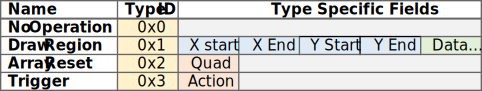
\includegraphics[width=1.0\textwidth]{fig/packet_chart.pdf}
        \caption{List of PDP Packets}
        \label{fig:packets}
    \end{figure}

    In terms of the protocol itself, PDP uses a single global coordinate system to refer to pixel locations on a display array. For example, a 512 by 512 pixel array would have coordinates from 0 to 511 in both the horizontal and vertical directions. All packets referencing sub-regions of this display would utilize coordinates that map to some rectangular sub-region of the display. Any overlapping regions of data would be composited during system operation with priority given to data segments sent at higher frame rates.

    PDP Packets are segmented into three types, a draw region packet, array reset packet, and trigger packet. All packets consist of a Type ID field of word-size. The draw region packet is used to send a rectangular sub-region of pixel data in global array coordinates. It has fields for the start and stop horizontal and vertical coordinates (defined inclusively) followed by individual pixel data. For example, suppose a scene generator were to send a packet of data from array region 10 to 19 along the X axis and 20 to 29 along the Y axis, a total of 100 pixels of data would follow the packet coordinates given that the packet specifies a 100 pixel sized region.

    The second packet, array reset, is utilized to indicate that quadrants on a given array should be cleared. It consists of an array specific quadrant bit-mask used to indicate which quadrant to reset. Any unused bits are reserved. This type of packet would be utilized exclusively between compositor and array tile links.

    The third packet, trigger, is used to implement a trigger based synchronization within in PDP. It consists of a system specific action bit-mask used to indicate the type of operation to trigger. In IRLED array systems, the coordinator of synchronization is dependent on the array itself and the different components within the system. In some systems, a sensor may be used as the source of synchronization, in other systems, another component may be utilized. Other aspects of system operation may even be triggered outside of the system synchronization interval based off of other events. For the reason, PDP has opted for a trigger based approach to synchronization. This approach allows for synchronization, data transfer, and computation to be custom tailored to an individual systems use-case. For example, the action mask could be used to trigger the generation of the next frame to be displayed when needed, the source of which is defined by the system itself. Another example would be utilize the action mask to indicate that further computations (such as scene generation) stall until otherwise indicated.

\section{PDP Frames}
    %FIXME: insert picture from slide 38 of real proposal

    \chapter{Machine Model}
        \label{chap:machine_model}

%FIXME: compare to slides 24-29 in REAL PROPOSAL
%FIXME: discuss PDP goal 1 here.

This chapter describes the abstract architecture upon which the PDP protocol operates in order to motivate current and future use cases. Additionally, a discussion of how different components operate within the system is provided for the reader to gain an intuition of the underlying operation.

%FIXME: remove "We"
Traditional IRLED display systems are typically composed of three components as part of the display: scene generation, non-uniformity correction, and the actual display of InfraRed with sensors used to capture data. This chapter proposes an Abstract Machine Model (AMM) to capture these three components as shown in Figure~\ref{fig:amm}. This AMM separates the system operation of an IRLED system into three main components as well: scene generation, compositing, and display on IRLED array tiles with links between each component. The relationship between these components remains abstracted in such a way that hardware components may be scaled to fit demand. At its most basic, a single scene generator, compositor, and IRLED array tile may be used. For higher speed requirements, hardware components may be mapped as needed. The links between components in the system utilize the PDP protocol for communication, data-transfer, and synchronization. The compositing component differs from a traditional IRLED system in that it is responsible for taking imagery from many sources, possibly at different frame rates, and combining them into a single image for transmission to IRLED array tiles. This process is briefly shown in Figure~\ref{fig:compositing}. During the compositing process frame segments are ranked to determine which to send at highspeeds, and which to send at low speeds for intelligent bandwidth utilization. Once segmented and ranked into non-overlapping speed classes, frame segments are transmits at the necessary rate.

\begin{figure}
    \centering
        \centering
        \includegraphics[width=0.83\textwidth]{fig/amm.pdf}
        \caption{Abstract Machine Model of the PDP architecture with 1-to-N relationships between components}
        \label{fig:amm}
\end{figure}

\begin{figure}
        \centering
        \includegraphics[width=1.0\textwidth]{fig/compositing.pdf}
        \caption{Compositing Process Example}
        \label{fig:compositing}
\end{figure}

\begin{figure}
        \centering
        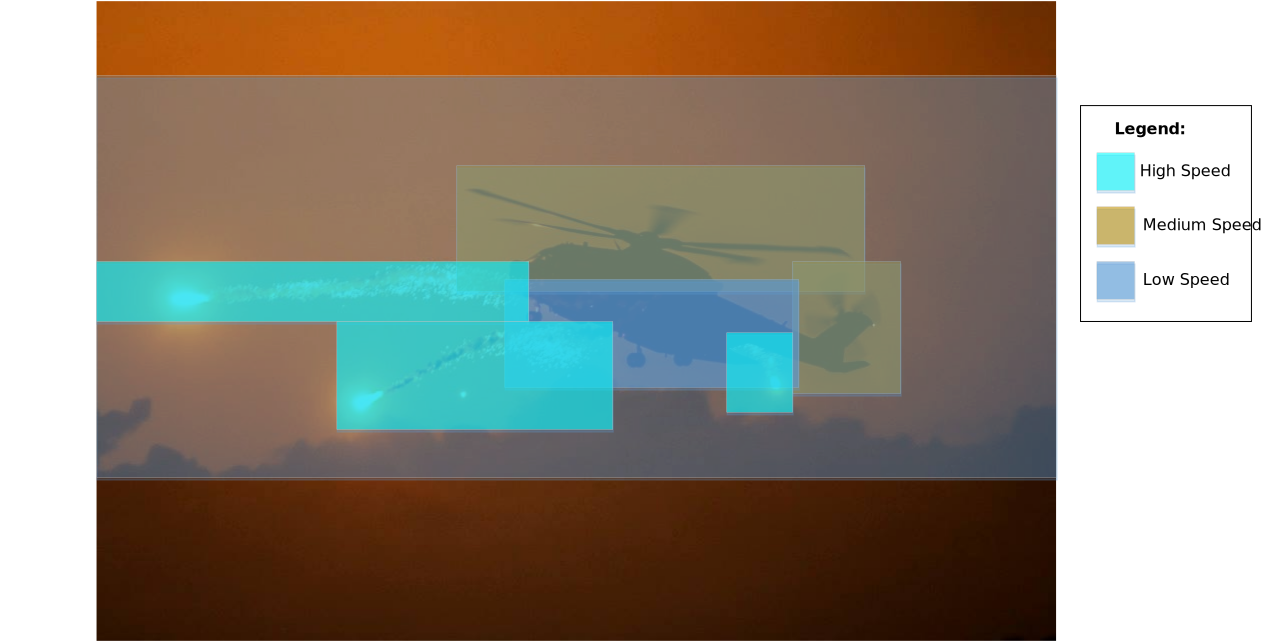
\includegraphics[width=1.0\textwidth]{fig/compositing_combined.pdf}
        \caption{Compositing Process Overlayed}
        \label{fig:compositing_overlayed}
\end{figure}

For example consider the simple case, that of a single scene generator. In this case, the compositor will receive data from a single source. As frame data is received, a differencing algorithm must be employed to determine how to segment the overall frame for optimal data transfer based off of the rate of change of individual portions of the frame relative to the prior frame. Portions that rapidly change will be sent more often than portions that change slowly in order to maximize bandwidth for high-speed transfer of {\it hot} portions of an image. This consequently also has the effect of improving the performance of the analog chain of display devices by allowing for devices to reserve more time to drive rapidly changing portions of a display over portions of the display changing relatively slowly.

    \chapter{Implementation}
        \label{chap:implementation}
%FIXME: V1 decoder logic
%FIXME: original SCB
%FIXME: Add information about the development history thingies from the repo
%FIXME: my research group's arrays?
%FIXME: talk about fw control modularity

%FIXME: fix this paragraph
This chapter describes an FPGA implementation of the PDP architecture~\cite{LandwehrEtAl2019_2,JacksonEtAl2019,BrowningEtAl2020}. For the purposes of this discussion, only relevant details are included to ease the readers understanding. First, the chapter will discuss the purpose of the implemented architecture. Following this each component will be discussed at a high-level. Finally, the operation of sub-components will be discussed.

\section{HDMI Transport Layer}
    \label{sec:hdmi_transport_layer}
    %FIXME: Discuss goal 4

    This section discusses utilizing HDMI as a transport layer for PDP. HDMI was chosen for the first implementation of PDP for several reasons. Firstly, current IRSP technology typically utilizes display protocols and the cooresponding links so from the perspective of hardware compatibility a display based protocol layer is ideal. Secondly, providing a backwards compatible implementation of PDP is a design goal as discussed in Chapter~\ref{sec:design_methodology}. Thirdly, utilizing existing hardware and systems is much cheaper and quicker than designing new hardware. Fourthly, minimizing barriers to entry for users of the protocol is important. Fifthly, it allows for a direct comparison with the same hardware. Sixthly, the systems in my lab utilize HDMI directly already.

    Recall that HDMI is a display protocol with blanking regions as discussed extensively in Chapter~\ref{sec:conventional_display_protocols}. Display protocols have an {\it Active Video} region as shown in Figure~\ref{fig:display_protocol_timing_overview}. This region is made up of scanlines that represent rows of pixels. In normal HDMI operation, the active video region is is simply representation of all visible pixels for a projector to display similar to when HDMI is utilized with a normal computer monitor. At the start of a frame, the first pixel will be streamed to an HDMI decoder and translated to an analog voltage to physically drive the first pixel of a display starting from the top left corner. Following this, subsequent pixels as streamed in and drive each pixel moving toward the right. When an hsync pulse occurs, the display moves to the next row and begins again. this is a typical rasterisation process.

    Traditional IRSP technology uses display protocols quite similarly but reorders data depending on how the rasterization process differs for the projector hardware. Recall the NSLEDS and HDILED array write process discussed in Chapter~\ref{sec:array_Interleaved_write_process} which includes a transpose and data reordering. For purposes of this discussion let us put aside any data reordering and blanking regions. Without lost of generality, drawing to an IRSP looks like Figure~\ref{fig:classic_video} where {\it D} represents an individual 24-bit pixel. Each {\it D} pixel would be decoded one by one as the data is streamed over HDMI to a decoder, and mapped to physical pixel on an array.

    \begin{figure}
        \centering
        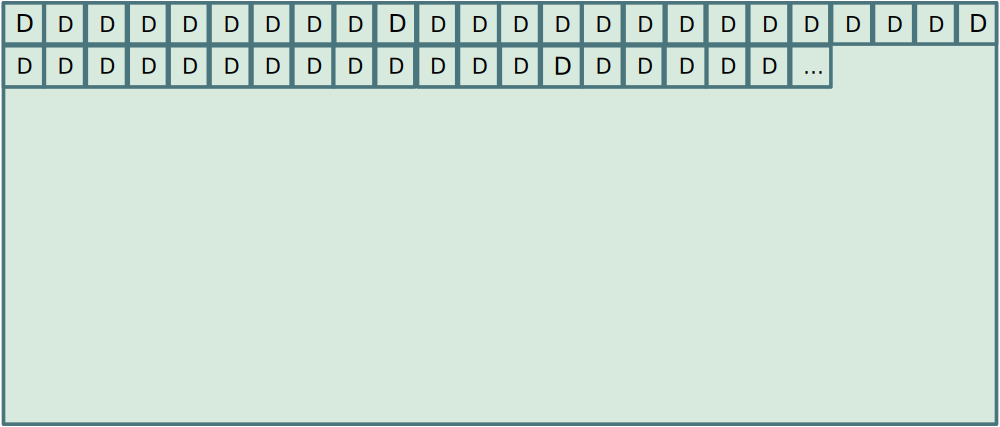
\includegraphics[width=1.0\textwidth]{fig/classic_video.pdf}
        \caption{Normal Frame with Display Data}
        \label{fig:classic_video}
    \end{figure}

    Now let us review the details of the PDP {\it Draw Region} packet shown in Figure~\ref{fig:packet_refresher}. Recall that it consist of an ID number, x start address, x end address, y start address, end y address, and trailing pixel data. The header data is denoted in yellow and the pixel data denoted in green. Recall additionally, that PDP allows its internal word size to be implementation specific; as such, for HDMI it is ideal to use a 24-bit word size in order to allow for fixed width pixel decoder logic. Additionally, this allows for each PDP word to be directly embeddable within an HDMI display stream with a one to one mapping between an HDMI pixel and a PDP word.

    \begin{figure}
        \centering
        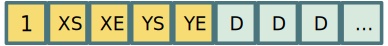
\includegraphics[width=0.5\textwidth]{fig/packet_refresher.pdf}
        \caption{Draw Region Packet}
        \label{fig:packet_refresher}
    \end{figure}

    Extrapolating, PDP region packets can be embedded into a HDMI data stream as shown in Figure~\ref{fig:embedded_frame} where each PDP word would be represented as a 24-bit pixel in the HDMI data stream. However, the meaning of the pixels differs from a normal frame in that only some pixels will be displayed to an array, and the location of displayed pixels is dependent on the header data preceding the pixels instead of using the start of the frame and the hsync regions to determine the location as is the case with normal HDMI. As the pixel words are streamed in, they are decoded one by one and examined for a context. For example, at the start of the example stream, an ID word would be streamed and decoded, signaling to the firmware that a Draw Region packet is being streamed in. From there, the four header words representing the region size would be streamed in, and stored for determining where to draw the pixel data that follows. As the pixel data is streamed in, the firmware would actively draw pixels in the cooresponding locations on the array where the header says the data should be located. This process would be continued until the end of a packet, and then the subsequent packet would undergo the same process.

    \begin{figure}
        \centering
        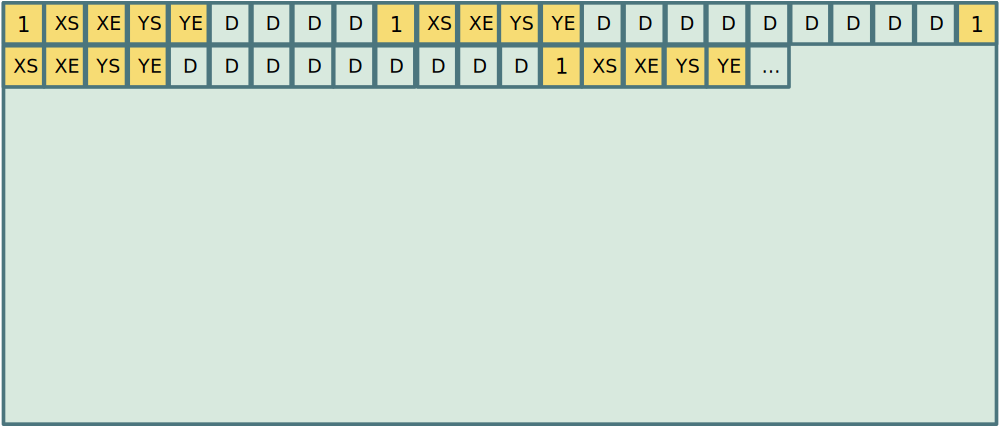
\includegraphics[width=1.0\textwidth]{fig/embedded_frame.pdf}
        \caption{Embedded PDP Frame}
        \label{fig:embedded_frame}
    \end{figure}

    This effectively separates the location a pixel is drawn at from the location in which it exist within an HDMI stream allowing for pixels to be driven independently of the HDMI stream resolution. Moreover, pixels can be driven more than one time within an embedded PDP frame by simply specifying another packet with the same overlapping locations. This allows for pixels to be driven at a faster rate then the base HDMI resolution. In fact, with the separation of pixel draw location from stream location, a specific HDMI resolution is not even necessary. Smaller faster resolutions can be utilized to draw arrays with larger resolutions than a modeline specifies as shown in Figure~\ref{fig:embedded_frame_to_emitter}. Ultimately, this allows for costume tailored modelines with different resolutions and base framerates to be utilizable with PDP over HDMI. Moreover, these benefits would hold for other display protocols if used as a PDP transport layer such as DisplayPort, and would allow PDP to be utilized by simply replacing the HDMI decoder hardware with other off the shelf decoder components without requiring changes to the PDP decoding logic or implementation, thus easing hardware requirements and vendor lock-in for PDP based implementations.

    \begin{figure}
        \centering
        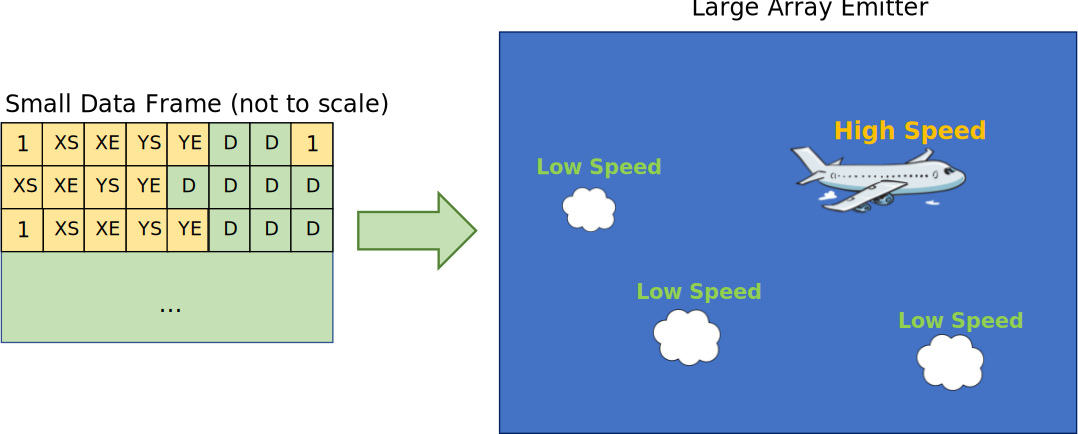
\includegraphics[width=1.0\textwidth]{fig/embedded_frame_to_emitter.pdf}
        \caption{Embedded PDP Frame to Array Mapping}
        \label{fig:embedded_frame_to_emitter}
    \end{figure}

    For backwards compatible operation with normal HDMI, one will note that a normal HDMI frame could be expressed as a single draw region packet with a header at the start the start of a frame. For purposes of backwards compatibility it is not necessary to send the header over HDMI itself. Instead, the header information could be sent as configuration information to PDP firmware and the HDMI data stream treated as normal display data. This allows for the same decoding and array write logic to be used both for embedded PDP frames and normal HDMI frames without requiring a separate implementation. Thus, users can operate the firmware in either a backwards compatible mode of operation or normal PDP mode of operation. Now that the format of data moving into PDP firmware has been discussed, the next section moves to a general discussion of the PDP firmware layout.

\section{Abstract Architecture}
    There are many important considerations when implementing a PDP based firmware for IRSPs. These range from pulling data into the FPGA over physical pins to clock domain crossing and timing issues.

    HDMI itself operates with a given pixel clock that's specified on the source side of the connection (at the machine generating the HDMI stream), meaning that the PDP firmware needs to support configurable HDMI speeds. The decoding of the HDMI stream itself is performed by off the shelf HDMI cards as noted in Chapter~\ref{sec:close_support_electronics}; therefore, the PDP firmware does not need to directly handle the protocol. Instead the firmware receives individual pixels at the pixel clock rate over two inputs simultaneously due to CSEs having two separate HDMI inputs.

    The array itself requires a specific timing for its signaling as well as enough time to completely settle any analog data lines; otherwise, pixels will flicker due to metastability issues with the signaling. This means that the HDMI clock cannot be directly utilized for timing array writes without introducing severe complications for correct timing. In fact, older non-PDP firmware implementations operated this way which resulted in image quality being negatively impacted at high speeds.

    In order to correct for these issues and guarantee stable operation at high speed, the PDP firmware implementation instead opted to isolate firmware operation into separate clock domains as shown in Figure~\ref{fig:abstract_architecture}. Ideally, there would simply be write and read clock domains where the write clock domain is clocked by the input HDMI pixel clock, and pixel data is buffered over an asynchronous boundary to the read clock domain. The read clock domain would operate at a static predefined speed that is faster than the write clock domain in order to ensure that under normal operation data cannot be lost. It would be responsible for decoding pixel data into headers and array data and drive an arrays signaling directly. In practice, the writer clock domain is separated into two separate clock domains for each HDMI input so that the HDMI input clocks do not need to be perfectly synchronized. As will be discussed shortly in subsequent sections, a correct and performant asynchronous boundary proved challenging in practice due to metastability issues and varability in FPGA synthesis from build to build.

    \begin{figure}
        \centering
        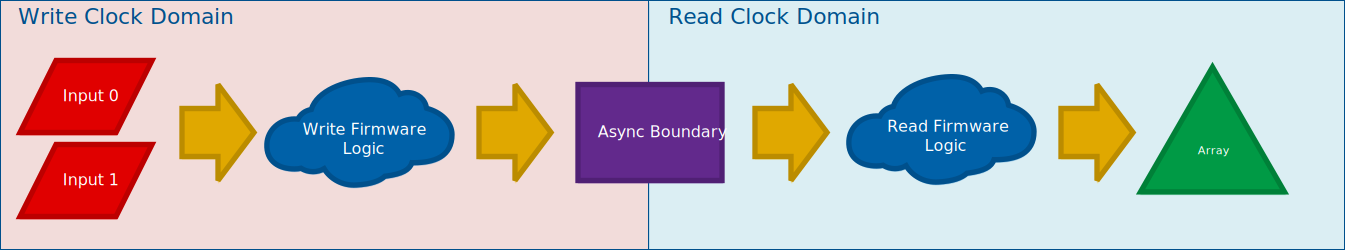
\includegraphics[width=1.0\textwidth]{fig/abstract_architecture.pdf}
        \caption{Abstract PDP Firmware Backend Architecture}
        \label{fig:abstract_architecture}
    \end{figure}

\section{Frontend Architecture}
    \label{sec:frontend_arch}
    This section will discuss the PDP frontend architecture. This is the portion of the firmware that is controllable and allows for user configuration. Recall from Figure~\ref{fig:cse_comm_block} in Chapter~\ref{sec:communication_flow} that CSE communication utilizes the cvorg protocol which is brought into a soft Microblaze soft-processor. PDP opted to retrofit this layer for its own configuration. Essentially, the frontend architecture works by decoding cvorg protocol commands which in turn set internal PDP registers which are read by the backend architecture for configuration. These include such things as controlling the length of time an individual array write occurs for, controlling delays in the signaling going to an array, and to control whether to operate the firmware in backwards compatibility mode where header data is read from internal PDP registers (called AXI mode) or PDP stream mode where header data is embedded into HDMI streams. Select APIs are shown in Table~\ref{tbl:apis}.

    \begin{table}
        \centering
        \small
        \begin{tabular}{| l l |}
            \hline
            API & Description \\ \hline
            get\_axi\_dimensions     & Gets AXI mode dimensions as 32-bit unsigned integers.        \\
            get\_axi\_mode           & Gets AXI mode. 0 is stream mode. 1 is backwards compat mode. \\
            get\_post\_write\_ticks  & Gets the post write duration for PDP.                        \\
            get\_state               & Gets current firmware state information.                     \\
            get\_write\_ticks        & Gets the delay and duration for pixel writes in PDP.         \\
            set\_axi\_dimensions     & Sets AXI dimensions.                                         \\
            set\_axi\_mode           & Sets AXI mode. 0 is stream mode. 1 is backwards compat mode. \\
            set\_error\_clear        & Sets clear bit for sticky error flags (overflow, stall).     \\
            set\_post\_write\_ticks  & Sets the post write duration for PDP.                        \\
            set\_write\_ticks        & Sets the delay and duration for pixel writes in PDP.         \\
            \hline
        \end{tabular}
        \caption{PDP Select Communication APIs}
        \label{tbl:apis}
        %\end{small}
    \end{table}

\section{Overall Backend Architecture}
    \label{sec:backend_arch}
    The implemented backend architecture consists of the portion of the AMM that drives an IRLED tile (or emitter array) directly from data packets sent by a compositor. As such, it is responsible for receiving PDP packets, decoding, validating, and drawing them to an IRLED array. This is shown in Figure~\ref{fig:overall_arch}. In the current implementation, packets are sent using an underlying HDMI protocol layer. The incoming data is synchronized across two distinct clock domains utilizing a synchronized circular buffer (SCB). The input side consists of two separate HDMI inputs to meet system bandwidth requirements. Each input is assumed to contain clock skew relative to the other so separate SCBs are used to synchronize these to the system domain. At a high-level, individual data words of 24-bit sized values come in per HDMI cycle. These are transitioned to the system domain and stored for retrieval by the array emitter module. The array emitter module is responsible for bringing in each 24-bit word value and emptying the corresponding SCB slot. As it brings in each word, it begins to decode them into PDP commands. Once enough data is buffered for a command, the data is sent to the write buffer module which then drives an emitter directly through I/O lines.

    \begin{figure}
        \centering
        \includegraphics[width=1.0\textwidth]{fig/pdp_overall_arch.pdf}
        \caption{Overall PDP Backend Architecture}
        \label{fig:overall_arch}
    \end{figure}

\section{Synchronized Circular Buffer}

    Figure~\ref{fig:scb_arch} shows the submodule details of the synchronized circular buffer utilized in the implementation. Internally, it consists of two controllers, two data routers, and the actual internal buffer storage with a built-in synchronizer circuit.

    \begin{figure}
        \centering
        \includegraphics[width=1.0\textwidth]{fig/pdp_scb_arch.pdf}
        \caption{Synchronized Circular Buffer Architecture}
        \label{fig:scb_arch}
    \end{figure}

    The write controller is used to coordinate which internal buffer to write data to. A buffer is marked as full when a write trigger comes in which in turn causes a new buffer to be selected in the same clock cycle. In terms of HDMI, when a pixel is streamed in, the HDMI write enable go high, clocking the pixel into the synchronized buffer and causing the buffer swap to occur. The write router performs the actual data redirection based off the buffer selected by the write controller. At high-level, internally, a request-acknowledgment handshake is used to ensure the data has transitioned correctly across clock domains and is available on the other side. The details of this implementation will be discussed in Chapter~\ref{Sec:MemorySync}. Once data becomes available, the read router will output the data lines as well as a valid signal indicating that the data can be read and cleared. The read controller will clear it once an empty trigger is sent from the array emitter indicating that the corresponding word has been read. It will then select the next buffer. Once the last buffer is written or read by either controller, the first buffer will be selected again. To note here for clarity, the actual filling and clearing of the buffers is done by HDMI write enable on the writer side, and the array emitter on the reader side.

    \subsection{Controllers}

    \subsection{Routing}

    \subsection{Internal Buffer and Memory Synchronizer}
    \label{Sec:MemorySync}

    Figure~\ref{fig:sb_arch} shows the internals of the internal buffers used by the SCB.
    \begin{figure}
        \centering
        \includegraphics[width=1.0\textwidth]{fig/pdp_sb_arch.pdf}
        \caption{Synchronized Internal Buffer Architecture}
        \label{fig:sb_arch}
    \end{figure}

    Figure~\ref{blah} shows the internals of the memory synchronizer utilized by the SCB architecture.

\section{Array Emitter}

    Figure~\ref{fig:ae_arch} shows the details of the array emitter module used in the implementation. Internally, the array emitter consists of individual controllers that each perform a particular role. Currently these are the write enable controller, which controls writing draw region packets; the reset controller, which controls the resetting process per frame; and the valid controller which does validation checks on the input to verify the correctness of packets. Each controller takes in similar input signals and produces similar output signals with some exceptions depending on the actual function of the individual controller module. On the input side, each controller takes in a valid and data line corresponding to an individual word of a PDP packet. Additionally, an active line is brought into each controller to indicate whether another controller module is active or not. This is used to ensure that other modules do not become active (for correctness purposes) while another is currently processing a packet. During an idle phase, the write enable and reset controllers will wait for a corresponding packet ID to come in.

    \begin{figure}
        \centering
        \includegraphics[width=1.0\textwidth]{fig/pdp_ae_arch.pdf}
        \caption{Array Emitter Architecture}
        \label{fig:ae_arch}
    \end{figure}


\section{Write Buffer}
     Figure~\ref{fig:wb_arch} shows the details of the write buffer architectures inputs and outputs along with important signaling to other modules. The write buffer is responsible for driving the I/O pins that go to the array.

    \begin{figure}
        \centering
        \includegraphics[width=1.0\textwidth]{fig/pdp_wb_arch.pdf}
        \caption{Write Buffer Architecture}
        \label{fig:wb_arch}
    \end{figure}

\section{State Machine}
    When a packet ID matching an operation handled by a given controller arrives, the corresponding controller will switch states and then wait for the rest of the incoming packet data to arrive. This is shown in Figure~\ref{fig:state_machine}. For example, item 3 shows each state machine waiting for a corresponding PDP OP code. If a draw region packet ID were to arrive, then the state machine would wait for the X start address, X end address, Y start address, and Y end address shown in item 4. Finally, the state machine would buffer the needed data for a write and move to the write state once all data has been buffered. In the write state it would send the data to the write buffer. If more data needs to be written for the PDP packet, it would then continue buffering the needed data, and wait for the write buffer to be idle to send the next set of data. The busy line in Figure~\ref{fig:ae_arch} indicates when the write buffer is in the process of writing to the array. This would continue until all data was written for the packet, finally proceeding to the idle state. The reset controller contains similar logic, but for the reset process. The valid controller is used to ensure that incorrect or corrupt packet data is cleared. If an invalid packet OP code arrives during an array emitter idle phase, the valid controller will simply empty the corresponding SCB slot. In future revisions, it will perform CRC checks on packet data to ensure the header and body are valid. The Active-Out, Active-In, and Select lines are used to coordinate which array emitter module has control over the write buffer. After an array write, normally an array emitter will signal the write buffer that it is ceding control to the other array emitter, but only in cases where the other array emitter is currently active and waiting to write.

    \begin{figure}
        \centering
        \includegraphics[width=1.0\textwidth]{fig/pdp_state_machine.pdf}
        \caption{PDP State Machine}
        \label{fig:state_machine}
    \end{figure}

    \chapter{Experimental Results}
        
\label{chap:experimental_results}

This chapter discusses a number of experimental results obtained using the implemented PDP firmware discussed in Chapter~\ref{chap:implementation}. Only select results are included. These were chosen because they provide direct evidence that the protocol and PDP firmware solves the challenges put forth in Chapter~\ref{chap:problem_formulation} and meets the design goals discussed in Chapter~\ref{sec:design_methodology}.

 Firstly, memory synchronizer operation is discussed and evaluated as correct clock domain crossing is an essential requirement for array operation. Secondly, overall firmware behavior is evaluated in both simulation and practice. Thirdly, packetized operation is evaluated. Finally, overall results are discussed to provide a summary of lessons learned during operational testing.

\section{Memory Synchronizer}

    This section describes the various tests performed on the full/empty memory synchronizer used within the PDP firmware to synchronize data transitioning across clock domains. First, it discusses simulation results obtained through a full behavioral simulation of the PDP firmware. Secondly, it discusses using the memory synchronizer in a test setup and the pitfalls that occurred with earlier implementations.

    \subsection{Simulation}
        Figure~\ref{fig:full_empty_sim} shows the simulated results of the full/empty memory synchronizer when transitioning to full and back to empty for a writer and reader operating at \mbox{35.75 megahertz} and \mbox{200 megahertz}, respectively. For discussion about each signal and the expected internal behavior see Chapter~\ref{sec:memorysync}. Each state transition in the simulation should look similar to the state transitions shown in Table~\ref{tbl:full_empty_circuit_states}.

        \begin{figure}[t]
            \centering
            \includegraphics[width=1.0\textwidth]{fig/full_empty_sim.png}
             \caption{Behavioral Simulation of a Single Pixel Being Buffered Through the Full/Empty Memory Synchronizer}
            \label{fig:full_empty_sim}
        \end{figure}

        The circuit holds a steady state until the {\it set full} signal is toggled for a single {\it write clock} cycle. On the next {\it write clock} cycle, the {\it req signal} transitions high and the {\it empty flag} transitions low. Then the data is moved to the {\it read clock} domain using the two flip-flop synchronizer scheme discussed in the implementation details. At the next rising edge of the {\it read clock}, the data is latched into {\it req internal} which is an internal metastable register. Due to the speed difference between write and read clock speed, the data latches into the register quickly. Following this, a cycle later, the data is clocked into {\it req reg} which completes the {\it read clock} domain transition causes the {\it full flag} to transition high.

        Once any corresponding buffer data is handled by the PDP firmware, the {\it set empty} signal is toggled for a single {\it read clock} cycle. This causes the {\it ack} signal to transition high. Then the data is moved to the {\it write clock} domain using the two flip-flop synchronizer scheme discussed in the implementation details. At the next rising edge of the {\it write clock}, the data is latched into {\it ack internal}. Following this, a cycle later, the data is clocked into {\it ack reg} which completes the {\it write clock} domain transition. Notice that it takes much longer to transition data from the {\it read clock} domain to the {\it write clock} domain than vice versa. This is due to the slow write clock.

        A {\it write clock} cycle later, {\it req} transitions low. Subsequently, it transitions to the {\it read clock} domain just as before. Following this, the {\it ack} line is lowered and transitions to the {\it write clock} domain just as before. At the same time, the {\it empty flag} transitions high, and the circuit is in the state it began in.

        This follows the expected state transitions from Table~\ref{tbl:full_empty_circuit_states} with the only notable distinction being that transitions across clock domains take different amounts of time depending on the destination.

        In practice, a complete double handshake takes many cycles to complete which could lead to undesired overflow behavior. In PDP, overflow issues are mitigated by allocating enough internal buffers to allow for there to always be a buffer available for a writer to fill.

        Additionally, the use of the two flip-flop synchronizer means that it takes more than a single {\it read clock} cycle for the {\it full flag} to raise; however, given that the pixels of an IRLED array take many {\it read clock} cycles to charge, this does not pose a problem. Moreover, in practice, the {\it full flag} transitions in between two to three cycles of the reader clock depending on where the rising edge of the reader clock falls relative to the transitioning of the {\it req} signal.

        Figure~\ref{fig:full_empty_row_sim} shows the simulated results of the full/empty memory synchronizer with multiple pixels being buffered through it for a writer and reader operating at \mbox{35.75 megahertz} and \mbox{200 megahertz}, respectively. The large gaps of time between transitions to full are due to there being multiple buffers available as discussed above. This indicates that at the simulated rates no overflow can occur. In practice, it would be possible for overflow to occur if the write clock speed was close to the read clock speed; however, due to the maximum possible write speed for HDMI only being \mbox{148.5 megahertz} and the hiding of clock domain crossing latency via multiple buffers, a \mbox{200 megahertz} input clock is sufficient for correct behavior.

        \begin{figure}[t]
            \centering
            \includegraphics[width=1.0\textwidth]{fig/full_empty_row_sim.png}
            \caption{Behavioral Simulation of Multiple Pixels Being Buffered Through the Full/Empty Memory Synchronizer}
            \label{fig:full_empty_row_sim}
        \end{figure}

    \subsection{Experimental Testing}
        \label{sec:experimental_testing}
        Testing the memory synchronizer on real hardware was an important consideration because behavioral simulations do not capture timing behavior accurately. In real hardware, noise, clock jitter, and variations in synthesis introduce unpredictable behavior that can lead designs to fail unexpectedly if they have inherent metastability issues.

        Testing was performed using a ZYBO development board~\cite{Digilent2016} hooked up as shown in Figure~\ref{fig:zybo_setup}. Image data consisting of 256 by 256 pixels operating at \mbox{250 hertz} was sent over from a NUCPC to a ZYBO board running an implementation of the synchronized circular buffer. VGA was used to provide loop-back for visual inspection. It is not possible to check for bit-level accuracy using a VGA device due to the analog nature of the interface so a UART device was used as an alternative (slow) path to read out internal image data. It was also used to collect statistical information such as the error bits for a given configuration and the amount of data that passed through the interface.

        \begin{figure}[t]
            \centering
            \includegraphics[width=0.40\textwidth]{fig/zybo_setup.pdf}
            \caption{ZYBO Test Setup}
            \label{fig:zybo_setup}
        \end{figure}

        For the first test, the synchronized circular buffer circuit was driven using the checkerboard input image shown in Figure~\ref{fig:checker_pattern}. This pattern was routed to the loop-back device for visual inspection. It was manually retrieved over UART and diffed with the original image to check for bit-level accuracy.

        \begin{figure}[t]
            \centering
            \includegraphics{fig/checker.png}
            \caption{Checkerboard Input Image}
            \label{fig:checker_pattern}
        \end{figure}

        For the second test, a dynamic CRC-like pattern was used to verify data accuracy directly. Segments of eight 8-bit random values where generated and then inserted into an HDMI stream twice as shown in Figure~\ref{fig:crc_like_buffer}. The pattern dynamic changed for every input frame. Figure~\ref{fig:random_noise} shows an example pattern. Internally, the test circuit would compare the results of the segments and log errors. UART was used to retrieve the error count.

        \begin{figure}[t]
            \centering
            \includegraphics[width=0.75\textwidth]{fig/crc_like_buffer.pdf}
            \caption{CRC-like 16-pixel Stream}
            \label{fig:crc_like_buffer}
        \end{figure}

        \begin{figure}[t]
            \centering
            \includegraphics{fig/random_noise.png}
            \caption{CRC-like Input Image}
            \label{fig:random_noise}
        \end{figure}

        The initial synchronizer circuit employed the design was able to pass behavioral simulation testing but during the above experimental testing exhibited bit-level errors. Upon careful analysis, it was discovered that the design contained metastability issues due to how signals are routed during synthesis. The early design employed a clock switching strategy within the memory synchronizer circuit. Essentially, the clock of the circuit was switched depending on whether the circuit was full or empty. In practice, this would randomly fail depending on how the circuit synthesized due to variability in routing per run which resulted in the timing delays between components changing unpredictably. This would ultimately lead to clock handoff being metastable and the circuit entering an inconsistent state. The final design discussed in this dissertation removes the clock switching circuitry and instead employs the double handshake design discussed in Chapter~\ref{sec:memorysync} in order to guarantee correct operation. The test patterns discussed above were able verify this.

\section{Firmware}
    This section discusses behavioral simulations of the PDP firmware implementation and experimental results obtained from running the firmware on actual IRLED arrays. The simulations serve to verify correct operational logic and the experimental results serve to validate the timing behavior of the implemented circuits.

    \subsection{Simulation}
    This section provides captures of a few simulation inputs and outputs to show how packets arrive and are processed by the PDP firmware architecture. Other isolated module and integrated simulations (not shown here) were performed to access behavioral operation of the PDP firmware implementation. Additional module level unit testing was performed as well.

    In Figure~\ref{fig:input_example} simulated HDMI is shown. When video data enable (write enable) transitions high words of data representing PDP packets start to stream in. These are indicated by packet ID, X start, X end, Y start, Y end, and Packet Data. Each word would be stored in an SCB slot as indicated in the previous section. The final piece of data indicated is a reset packet. Note, that the data prior to Packet ID would be ignored as it does not represent a valid PDP command. It would be discarded by the valid controller.

    \begin{figure}
        \centering
        \includegraphics[width=1.0\textwidth]{fig/pdp_input_example.png}
        \caption{Simulation of Single HDMI Input}
        \label{fig:input_example}
    \end{figure}

    Figure~\ref{fig:output_example} shows the final output driven to the array. Highlighted in red is data from the write enable packet. Note, all values out are up shifted by 5 bits to be received by the DACs in the system. Additionally, the values are shown in reverse order from the input diagram. For example, 992 corresponds to the value of 31 on the input side. In purple the reset packet is shown with two stages of array writes. In the first stage, load line goes low. In the second stage the load line transitions high. The states shown are the transitioning of the state machines discussed in Chapter~\ref{sec:state_machines}.

    \begin{figure}
        \centering
        \includegraphics[width=1.0\textwidth]{fig/pdp_output_example.png}
        \caption{Simulation of PDP Output}
        \label{fig:output_example}
    \end{figure}

    \subsection{Characterization}
        This section shows select results of running the PDP firmware on an NSLEDS array to characterize its behavior. Namely, whether it correctly draws to an array and whether it performs better than earlier firmware incarnations. Some non-uniformity correct imagery is also shown which indicates the PDP firmware is capable of drawing full imagery correctly. Though, only a few results are shown here, the PDP firmware has been run on multiple NSLEDS and HDILED arrays to collect data and characterize the arrays themselves. As of this writing, it has been used in daily operations with my research group's IRLED arrays for over a year and is the primary firmware in use today.

        \subsubsection {Array Maps}
            In order to characterize whether the behavior of the PDP firmware is consistent with older firmware (called SNAP) and has reproducible results between runs, a number of different array characterization tests were performed on an NSLEDS array. One test is to collect an array map which is performed by doing a sweep of array pixels by outputting light to each pixel separately over multiple frames and capturing the result. Typically, this is done using grids to speed up data collection. An example grid for a partial frame is shown in Figure~\ref{fig:grid_sweep}. Defective pixels on an array have low light output or have inconsistent brightness from run to run. This could also happen if a firmware contained internal timing issues as well. Comparing a test firmware with a known good reference firmware can rule out firmware issues in the advent of this type of poor array behavior.

            \begin{figure}[t]
                \centering
                \includegraphics{fig/grid.jpg}
                \caption{Pixel Sweep Grid}
                \label{fig:grid_sweep}
            \end{figure}

            Figure~\ref{fig:array_map_pdp} shows an array map collected from the PDP firmware and Figure~\ref{fig:array_map_snap} shows an array map collected from the older SNAP firmware. In each figure, array data collected using an IR camera is shown on the left with a camera count scale on the right. Camera counts are an uncalibrated measure of IR intensity that can mapped to apparent temperature when calibrated. At a glance, each image appears to be the same; however, PDP firmware has a slightly higher light output. The dark regions of each map are dead pixels on the array and do not reflect the firmware. More than half of the particular array is nonfunctioning. The repeating patterns of horizontal lines that can be seen are the result of slow DAC channels on an array. Every 32 columns there are 2 channels which take longer to settle and that can be seen in these results, as these channels have not fully settled. This is due to design flaw on early arrays which resulted in higher capacitance on those lines. Overall, the PDP firmware results are as expected and indicate correct operation.

            \begin{figure}[t]
                \centering
                \includegraphics[width=1.0\textwidth]{fig/array_map_pdp.jpg}
                \caption{Array Map of PDP Firmware Output}
                \label{fig:array_map_pdp}
            \end{figure}

            \begin{figure}[t]
                \centering
                \includegraphics[width=1.0\textwidth]{fig/array_map_snap.jpg}
                \caption{Array Map of SNAP Firmware Output}
                \label{fig:array_map_snap}
            \end{figure}

        \subsubsection{Fractional Difference Maps}

            Another test is to collect multiple array maps and take the fractional difference between them to see the percent difference in light output between runs. This allows for the consistency of light output to be characterized. A large difference could indicate problems with the pixels of an array, analog chain, or firmware behavior. Small differences indicate that the pixels of an array are more consistent between runs. Differences in behavior between firmware (or firmware revisions) would be indicative of variance in signal timing. In this case, a larger variance would indicate less precise timing within the firmware. Some variance is expected is due to camera focus, noise, and physical vibration. The particular IR camera used to collect data in this setup utilizes a motorized reversed-stirling cryo-cooler. These are often utilized for cooling detectors within thermal imaging systems~\cite{Organ1999}. These induce a physical vibration which can result in noise within collected camera imagery.

            Figure~\ref{fig:fractional_difference_pdp} shows a fractional difference map for the PDP firmware and Figure~\ref{fig:fractional_difference_snap} shows a fractional difference map for the older SNAP firmware. The dark blue areas indicating zero difference are dead regions of the array similar to the earlier results. The red areas of high variance are due to those pixels being located on marginal portions of the array specifically along non-functioning edges. In practice for displaying imagery, these areas would be marked as defected and not driven.

            \begin{figure}[t]
                \centering
                \includegraphics[width=1.0\textwidth]{fig/fractional_difference_pdp.jpg}
                \caption{Fractional Difference Map of PDP Firmware Output}
                \label{fig:fractional_difference_pdp}
            \end{figure}

            \begin{figure}[t]
                \centering
                \includegraphics[width=1.0\textwidth]{fig/fractional_difference_snap.jpg}
                \caption{Fractional Difference Map of SNAP Firmware Output}
                \label{fig:fractional_difference_snap}
            \end{figure}

            The average variance for both the SNAP and PDP firmware is less than 4 percent. However, the PDP firmware has less variance in per pixel light output per run as indicated by the darker blue colors in the working portions of the array compared to the SNAP firmware. This is likely due to the static \mbox{200 megahertz} system clock used for driving an arrays pixels combined with the two flip-flop synchronization strategy utilized within the PDP firmware that is discussed in Chapter~\ref{sec:memorysync}. The earlier SNAP firmware used an HDMI clock signaling based approach to time triggering of events on the system side. Given that the clock is an input from an external HDMI card, it most likely has some noise. Another factor that may contribute to the larger variance is the fact that most functionality within SNAP used only the first HDMI card clock and ignored the second HDMI card clock. The crystal oscillators used for generating clock signals within devices typically has a finite precision due to various contributing factors such as thermal noise, power supply variations, and aging~\cite{Naval2002}. This means that oscillators within the same device model may vary resulting in clock skew. Any inherit oscillation skew could be further compounded by the fact that each HDMI cards data lines travel physically different trace paths to arrive within the FPGA. The PDP firmware on the other hand, makes no assumptions about input clock skew. The Memory synchronizer utilized within explicitly synchronizes the data of each HDMI card separately across clock domains to the system clock domain. Then it explicitly pulls data from each synchronized circular buffer independently. Overall, the behavioral results are promising for the PDP firmware.

        \subsubsection{Non-uniformity Corrected Imagery}
            Figure~\ref{fig:pdp_bird} shows an example of non-uniformity corrected IR imagery generated using the PDP firmware on an NSLEDS array. This particular array has much better yield than the one used for some of the earlier results presented in this chapter and is capable of displaying full images at a 1024 by 1024 resolution.

            \begin{figure}[t]
                \centering
                \includegraphics{fig/pdp_bird.png}
                \caption{Still Image Capture of a Non-uniformity Corrected Image from the PDP Firmware Operating at 100Hz}
                \label{fig:pdp_bird}
            \end{figure}

            Figure~\ref{fig:pdp_grid} shows a grid being displayed on the same array. The lower right-hand corner of the array has physical defects, but the majority of the array operates correctly. Interspersed in between the working pixels are a couple of dead pixels here and there. These look worse in a static grid map than in practice, as the brightness of neighboring pixels effectively hides individually defective pixels within an array. This is true as long as multiple pixels within a small region of an array are not defective as well. This is why Figure~\ref{fig:pdp_bird} shows no obvious dead pixels even though individual pixels are defective within the region that the image is displayed on.

            \begin{figure}[t]
                \centering
                \includegraphics[width=0.76\textwidth]{fig/pdp_grid.png}
                \caption{Still Image Capture of a Grid from the PDP Firmware Operating at 100Hz}
                \label{fig:pdp_grid}
            \end{figure}

        \subsubsection{Analog Bandwidth}
            \label{sec:analog_bandwidth}
            Figure~\ref{fig:pdp_bird_comparison} shows the same IR image drawn at two different frame rates using the PDP firmware operating in backwards compatibility mode. In this mode, normal HDMI data is sent to an array at full resolution. At \mbox{100 hertz} operation, the image quality is much more uniform across pixels despite having low dynamic range when not non-uniformity corrected. At \mbox{400 hertz} operation there are distinct banding patterns that are not visible at lower frame rate. These banding patterns are the result of limited analog bandwidth due to the time it takes for the analog portions of the system to settle which includes DAC settling time, amplifier settling time, RIIC internal timings, and emitter charge time. Under normal HDMI operation it is difficult to correct for these issues at high-speed without introducing complicated compensation schemes such as analog or digital pre-emphasis filtering\footnote{Analog and digital pre-emphasis is used in many types of applications~\cite{BuckwalterEtAl2006, RafiqueEtAl2015, HuEtAl2017, ThaiEtAl2018, ZhouEtAl2020}}.

            \begin{figure}[t]
                \centering
                \includegraphics[width=1.0\textwidth]{fig/pdp_bird_comparison.png}
                \caption{Comparison of Imagery Captured from the PDP Firmware Operating at 100hz and 400hz}
                \label{fig:pdp_bird_comparison}
            \end{figure}

            Utilizing a packetized approach to display can help mitigate issues with high-speed display by providing more time for changing regions of a display to settle. Consider a 1024 by 1024 display operating at high speed. When packetized operation is utilized, ideally only subregions of the display are updated at high-speed and the portions of the array operating at low-speed are addressed at much slower rate; and thus, use much less analog bandwidth. The exact amount of analog bandwidth saved would depend on how much of the imagery needs to run at high-speed; however, this could on the order of a 75 percent reduction in cases of low-speed backgrounds with small high-speed objects. This means that portions updating at high speed can be driven for longer amounts of times to allow for complete settling.

\section{Packetized Operation}
        This section shows various examples of the PDP firmware running at low-speed and high-speed operation to demonstrate the capabilities and versatility of a packetized display protocol. Additionally, multiple frame rate operation is demonstrated at high-speeds to show the capabilities of packetized operation.

    \subsection{Normal-speed}
        Figure~\ref{fig:low_speed_numbers} shows a series of counting numbers operating at low speeds. These were part of some of the initial demos used for testing packetized operation. This demo, in particular, ran at a number of different rates ranging from \mbox{60 hertz} to \mbox{240 hertz} operation. It was used as an initial verification of the firmware's packetized mode of operation.

        \begin{figure}[t]
            \centering
            \includegraphics[width=0.15\textwidth]{fig/low_speed_numbers.png}
            \caption{Still Image Capture of Counting Numbers from the PDP Firmware Operating at 60Hz}
            \label{fig:low_speed_numbers}
        \end{figure}

        Other imagery included moving objects across the array at low-speed and moving changing numbers. Of particular interest was analyzing the boundaries of each packet for artifacts in overlapping packet regions and verifying that moving objects were not exhibiting partial display of previous packet data as these behaviors may indicate incorrect firmware operation. In initial testing, some implementation challenges included ensuring that the correct packet data was being sent from the driving computer to the CSE and verifying that the correct pixels were being addressed from within the firmware. The former was addressed by attaching the HDMI output links to loop-back capture devices and meticulously analyzing the output to ensure both the data ordering described in Chapter~\ref{sec:data_ordering} was being abided by, and that packet headers were being correctly specified. The latter was addressed by analyzing the address lines routed directly to the array via oscilloscope.

    \subsection{High-speed}
        There have been a number of different high-speed demos used to test the PDP firmware at rates above \mbox{250 hertz} operation on an NSLEDS array. Due to the limitations in IR Camera speed, these were obtained by windowing the camera resolution down to allow for faster capture. Under full resolution, the IR cameras used can only reach \mbox{565 hertz} or \mbox{132 hertz} depending on the exact model.

        Figure~\ref{fig:high_speed_object} shows a still image for a demo of an object that moves along both the x and y dimensions of the array at \mbox{1 kilohertz}. When an edge is reached, the object bounces similar to the electronic game of Pong\cite{Alcorn1972}. This object was drawn using multiple PDP draw region packets embedded into a larger HDMI frame. For every packet, the {\it x start} and {\it y start} locations were modified. Drawing at this rate with normal full frame HDMI is impossible. At best, \mbox{240 hertz} may be used with sacrifices in image brightness due to limited analog bandwidth as discussed in Chapter~\ref{sec:analog_bandwidth}.

        \begin{figure}[t]
            \centering
            \includegraphics[width=0.15\textwidth]{fig/high_speed_object.png}
            \caption{Still Image Capture of a Moving Object from the PDP Firmware Operating at 1Khz}
            \label{fig:high_speed_object}
        \end{figure}

        Figure~\ref{fig:high_speed_numbers} shows a series of images for a number counting demo running at {2 kilohertz} operation. This demo consisted of both a static configuration in which a predefined location was used to display the number and moving configuration in which the number would move around the array in both the x and y dimensions. In both configurations, the number would increment by one at the given frame rate. The object itself was drawn using individual PDP packets for each numerical digit. As with the previous example, drawing at this rate with normal full frame HDMI is impossible which demonstrates that packetized operation can achieve rates well beyond normal HDMI with the same hardware.

        \begin{figure}[t]
            \centering
            \includegraphics[width=0.7\textwidth]{fig/high_speed_numbers.png}
            \caption{Still Image Captures of a Counting Number from the PDP Firmware Operating at 2Khz}
            \label{fig:high_speed_numbers}
        \end{figure}

        Figure~\ref{fig:high_speed_rotating_object} shows a series of frames for a non-uniformity corrected rotating three-dimensional object running at {2 Kilohertz} operation. The object itself was drawn using individual PDP packets for each rotation. Notably, even with the limited resolution of the IR camera when operating at a high-speed, the object is clear and distinct during each rotation. This demonstrates that packetized operation can indeed mitigate issues with limited analog bandwidth as discussed in Chapter~\ref{sec:analog_bandwidth}. A small object such as this could be displayed with a slow-speed background without sacrificing image quality which representative of some types of IR imagery used in practice.

        \begin{figure}[t]
            \centering
            \includegraphics[width=0.7\textwidth]{fig/high_speed_rotating_object.png}
            \caption{Still Images Captures of a Non-uniformity Corrected Rotating Object from the PDP Firmware Operating at 2Khz}
            \label{fig:high_speed_rotating_object}
        \end{figure}

    \subsection{Multi-frame Rate}
        Figure~\ref{fig:pdp_multi_frame_rate} shows a series of frames for a multi-frame rate display of numbers using the PDP firmware. The small bright number was updated at \mbox{800 hertz}, the small background numbers was updated at \mbox{100 hertz}, and the large number was updated at \mbox{2 hertz}. Each number was drawn using individual PDP region packets. Similar to other demos discussed in this chapter, each number was incremented at the corresponding frame rate. This demonstrates that multiple framerate display operates correctly within the firmware and is able to achieve rates much higher than possible with the same hardware utilizing conventional display technology.

        \begin{figure}[t]
            \centering
            \includegraphics[width=0.80\textwidth]{fig/pdp_multi_frame_rate.jpg}
            \caption{Still Image Captures of a Bouncing Number, Small Background Numbers, and a Large Number from the PDP Firmware Operating at 800Hz, 100Hz, and 2Hz, Respectively}
            \label{fig:pdp_multi_frame_rate}
        \end{figure}

\section{Summary}
    The demonstrations of packetized display protocol operation provided within this chapter make a strong argument to the benefit of this type of technology for use in future high-speed IRSP systems. This chapter presented a number of demonstrations of the PDP firmware running on real hardware in various types of operation. A wide breadth of different experiments was shown including normal backwards compatible HDMI operation, low-speed packetized display, high-speed packetized display, and high-speed multiple frame rate operation.

    Taken together, these demonstrate that packetized operation is capable of vastly improving performance with various types of imagery in bandwidth starved environments. The improvements in digital bandwidth utilization from packetized operation show that substantially higher frame rates can be achieved. Additionally, multiple frame rate operation, in particular, enables better analog performance by allowing analog bandwidth to be to be reserved for high-speed updates of pixel regions which in turn yields improved overall image quality. In contrast, conventional display technology requires that analog bandwidth be apportioned equally for all pixels which results in considerably inferior image quality at high-speeds.

    The subsequent and final chapter of this dissertation is devoted to an overall discussion of the journey through the architectural development and implementation of a packetized display protocol architecture for infrared scene projection systems.

    \chapter{Conclusion}
        %FIXME: remove "we"
\label{chap:conclusion}
In this paper, we described a packetized display protocol architecture and associated abstract machine model to convey the limitations in current fixed frame technology. Additionally, we provide an alternative display architecture that eschews the design decisions of current technology in order to provide intelligent dynamic bandwidth utilization, fine-grained control over frame transmission and synchronizationas well as allows for dynamically changing intra-frame rates. We believe this architecture has the potential to provide the capabilities to bridge the performance gap found in current technology, and will serve as a better-fit solution for future high performance IRLED systems due to the scalable nature of the design and the carefully incorporated abstraction tailored to allow for different types of hardware and system setups to utilize the PDP architecture. Care has been taken in the design to incorporate many different possible system setups without limiting the use case of PDP to a specific hardware setup; while at the same time, considering firmware implementation and timing aspects to packet decoding.

Current work includes a FPGA based implementation of a PDP decoder architecture utilizing HDMI. We have provided both a description of the implemented architectureas well as simulated sample data running on the architecture. Future work includes testing the architecture on an emitter array, performing scalability testing, and comparing the results to a conventional architecture at matching pixel clock rates in order to show effective speedup with varying packet sizes. Further work is to be done to demonstrate dynamic frame rates in action on an array. Finally, a CRC is to be implemented to ensure correct operation at all times. We also wish to scale the number of inputs in order to increase the effective hardware bandwidth further than capable with a conventional system.


    \renewcommand{\bibname}{References}
    \pdfstringdefDisableCommands{\let\uppercase\relax}
    \bibliography{bib/biblio}
    \bibliographystyle{unsrt}


\end{document}
